\documentclass[]{book}
\usepackage{lmodern}
\usepackage{amssymb,amsmath}
\usepackage{ifxetex,ifluatex}
\usepackage{fixltx2e} % provides \textsubscript
\ifnum 0\ifxetex 1\fi\ifluatex 1\fi=0 % if pdftex
  \usepackage[T1]{fontenc}
  \usepackage[utf8]{inputenc}
\else % if luatex or xelatex
  \ifxetex
    \usepackage{mathspec}
  \else
    \usepackage{fontspec}
  \fi
  \defaultfontfeatures{Ligatures=TeX,Scale=MatchLowercase}
\fi
% use upquote if available, for straight quotes in verbatim environments
\IfFileExists{upquote.sty}{\usepackage{upquote}}{}
% use microtype if available
\IfFileExists{microtype.sty}{%
\usepackage{microtype}
\UseMicrotypeSet[protrusion]{basicmath} % disable protrusion for tt fonts
}{}
\usepackage[margin=1in]{geometry}
\usepackage{hyperref}
\hypersetup{unicode=true,
            pdftitle={Applied Time Series Analysis},
            pdfauthor={Vipul Bhatt},
            pdfborder={0 0 0},
            breaklinks=true}
\urlstyle{same}  % don't use monospace font for urls
\usepackage{natbib}
\bibliographystyle{apalike}
\usepackage{color}
\usepackage{fancyvrb}
\newcommand{\VerbBar}{|}
\newcommand{\VERB}{\Verb[commandchars=\\\{\}]}
\DefineVerbatimEnvironment{Highlighting}{Verbatim}{commandchars=\\\{\}}
% Add ',fontsize=\small' for more characters per line
\usepackage{framed}
\definecolor{shadecolor}{RGB}{248,248,248}
\newenvironment{Shaded}{\begin{snugshade}}{\end{snugshade}}
\newcommand{\KeywordTok}[1]{\textcolor[rgb]{0.13,0.29,0.53}{\textbf{#1}}}
\newcommand{\DataTypeTok}[1]{\textcolor[rgb]{0.13,0.29,0.53}{#1}}
\newcommand{\DecValTok}[1]{\textcolor[rgb]{0.00,0.00,0.81}{#1}}
\newcommand{\BaseNTok}[1]{\textcolor[rgb]{0.00,0.00,0.81}{#1}}
\newcommand{\FloatTok}[1]{\textcolor[rgb]{0.00,0.00,0.81}{#1}}
\newcommand{\ConstantTok}[1]{\textcolor[rgb]{0.00,0.00,0.00}{#1}}
\newcommand{\CharTok}[1]{\textcolor[rgb]{0.31,0.60,0.02}{#1}}
\newcommand{\SpecialCharTok}[1]{\textcolor[rgb]{0.00,0.00,0.00}{#1}}
\newcommand{\StringTok}[1]{\textcolor[rgb]{0.31,0.60,0.02}{#1}}
\newcommand{\VerbatimStringTok}[1]{\textcolor[rgb]{0.31,0.60,0.02}{#1}}
\newcommand{\SpecialStringTok}[1]{\textcolor[rgb]{0.31,0.60,0.02}{#1}}
\newcommand{\ImportTok}[1]{#1}
\newcommand{\CommentTok}[1]{\textcolor[rgb]{0.56,0.35,0.01}{\textit{#1}}}
\newcommand{\DocumentationTok}[1]{\textcolor[rgb]{0.56,0.35,0.01}{\textbf{\textit{#1}}}}
\newcommand{\AnnotationTok}[1]{\textcolor[rgb]{0.56,0.35,0.01}{\textbf{\textit{#1}}}}
\newcommand{\CommentVarTok}[1]{\textcolor[rgb]{0.56,0.35,0.01}{\textbf{\textit{#1}}}}
\newcommand{\OtherTok}[1]{\textcolor[rgb]{0.56,0.35,0.01}{#1}}
\newcommand{\FunctionTok}[1]{\textcolor[rgb]{0.00,0.00,0.00}{#1}}
\newcommand{\VariableTok}[1]{\textcolor[rgb]{0.00,0.00,0.00}{#1}}
\newcommand{\ControlFlowTok}[1]{\textcolor[rgb]{0.13,0.29,0.53}{\textbf{#1}}}
\newcommand{\OperatorTok}[1]{\textcolor[rgb]{0.81,0.36,0.00}{\textbf{#1}}}
\newcommand{\BuiltInTok}[1]{#1}
\newcommand{\ExtensionTok}[1]{#1}
\newcommand{\PreprocessorTok}[1]{\textcolor[rgb]{0.56,0.35,0.01}{\textit{#1}}}
\newcommand{\AttributeTok}[1]{\textcolor[rgb]{0.77,0.63,0.00}{#1}}
\newcommand{\RegionMarkerTok}[1]{#1}
\newcommand{\InformationTok}[1]{\textcolor[rgb]{0.56,0.35,0.01}{\textbf{\textit{#1}}}}
\newcommand{\WarningTok}[1]{\textcolor[rgb]{0.56,0.35,0.01}{\textbf{\textit{#1}}}}
\newcommand{\AlertTok}[1]{\textcolor[rgb]{0.94,0.16,0.16}{#1}}
\newcommand{\ErrorTok}[1]{\textcolor[rgb]{0.64,0.00,0.00}{\textbf{#1}}}
\newcommand{\NormalTok}[1]{#1}
\usepackage{longtable,booktabs}
\usepackage{graphicx,grffile}
\makeatletter
\def\maxwidth{\ifdim\Gin@nat@width>\linewidth\linewidth\else\Gin@nat@width\fi}
\def\maxheight{\ifdim\Gin@nat@height>\textheight\textheight\else\Gin@nat@height\fi}
\makeatother
% Scale images if necessary, so that they will not overflow the page
% margins by default, and it is still possible to overwrite the defaults
% using explicit options in \includegraphics[width, height, ...]{}
\setkeys{Gin}{width=\maxwidth,height=\maxheight,keepaspectratio}
\IfFileExists{parskip.sty}{%
\usepackage{parskip}
}{% else
\setlength{\parindent}{0pt}
\setlength{\parskip}{6pt plus 2pt minus 1pt}
}
\setlength{\emergencystretch}{3em}  % prevent overfull lines
\providecommand{\tightlist}{%
  \setlength{\itemsep}{0pt}\setlength{\parskip}{0pt}}
\setcounter{secnumdepth}{5}
% Redefines (sub)paragraphs to behave more like sections
\ifx\paragraph\undefined\else
\let\oldparagraph\paragraph
\renewcommand{\paragraph}[1]{\oldparagraph{#1}\mbox{}}
\fi
\ifx\subparagraph\undefined\else
\let\oldsubparagraph\subparagraph
\renewcommand{\subparagraph}[1]{\oldsubparagraph{#1}\mbox{}}
\fi

%%% Use protect on footnotes to avoid problems with footnotes in titles
\let\rmarkdownfootnote\footnote%
\def\footnote{\protect\rmarkdownfootnote}

%%% Change title format to be more compact
\usepackage{titling}

% Create subtitle command for use in maketitle
\newcommand{\subtitle}[1]{
  \posttitle{
    \begin{center}\large#1\end{center}
    }
}

\setlength{\droptitle}{-2em}

  \title{Applied Time Series Analysis}
    \pretitle{\vspace{\droptitle}\centering\huge}
  \posttitle{\par}
    \author{Vipul Bhatt}
    \preauthor{\centering\large\emph}
  \postauthor{\par}
      \predate{\centering\large\emph}
  \postdate{\par}
    \date{2019-05-07}

\usepackage{booktabs}
\usepackage{amsthm}
\DeclareMathOperator*{\argmin}{argmin}
\DeclareMathOperator*{\argmax}{argmax}
\makeatletter
\def\thm@space@setup{%
  \thm@preskip=8pt plus 2pt minus 4pt
  \thm@postskip=\thm@preskip
}
\makeatother

\usepackage{amsthm}
\newtheorem{theorem}{Theorem}[chapter]
\newtheorem{lemma}{Lemma}[chapter]
\newtheorem{corollary}{Corollary}[chapter]
\newtheorem{proposition}{Proposition}[chapter]
\newtheorem{conjecture}{Conjecture}[chapter]
\theoremstyle{definition}
\newtheorem{definition}{Definition}[chapter]
\theoremstyle{definition}
\newtheorem{example}{Example}[chapter]
\theoremstyle{definition}
\newtheorem{exercise}{Exercise}[chapter]
\theoremstyle{remark}
\newtheorem*{remark}{Remark}
\newtheorem*{solution}{Solution}
\let\BeginKnitrBlock\begin \let\EndKnitrBlock\end
\begin{document}
\maketitle

{
\setcounter{tocdepth}{1}
\tableofcontents
}
\hypertarget{preface}{%
\chapter*{Preface}\label{preface}}
\addcontentsline{toc}{chapter}{Preface}

These lecture notes are prepared for an upper level undergraduate course in time series econometrics. Every fall I teach a course on applied time series analysis at James Madison University. These notes borrow heavily from the teaching material that I have developed over several years of instruction of this course.

One of my main objective is to develop a primer on time series analysis that is more accessible to undergraduate students than standard textbooks available in the market. Most of these textbooks in my opinion are densely written and assume advanced mathematical skills on the part of our students. Further, I have also struggled with their topic selection and organization. Often I end up not following the chapters in order and modify content (by adding or subtracting) to meet my students needs. Such changes causes confusion for some students and more importantly discourages optimal use of the textbook. Hence, this is an undertaking to develop a primer on time series that is accessible, follows a more logical sequencing of topics, and covers content that is most useful for undergraduate students in business and economics.

\emph{Note: These notes have been prepared by me using various sources, published and unpublished. All errors that remain are mine.}

\hypertarget{intro}{%
\chapter{Introduction to Forecasting}\label{intro}}

\hypertarget{time-series}{%
\section{Time Series}\label{time-series}}

A time series is a specific kind of data where observations of a variable are recorded over time. For example, the data for the U.S. GDP for the last 30 years is a time series data.

Such data shows how a variable is changing over time. Depending on the variable of interest we can have data measured at different frequencies. Some commonly used frequencies are intra-day, daily, weekly, monthly, quarterly, semi-annual and annual. Figure \ref{fig:ch1-figure1} below plots data for quarterly and monthly frequency.

\begin{figure}

{\centering 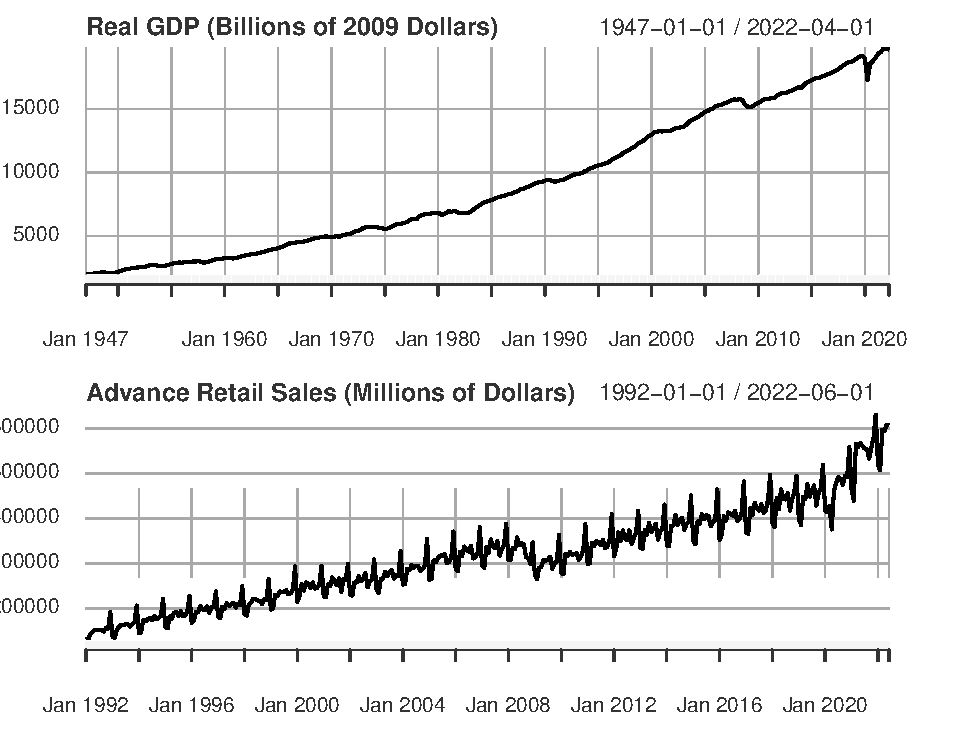
\includegraphics[width=0.8\linewidth]{bookdown-demo_files/figure-latex/ch1-figure1-1} 

}

\caption{Time Series at quarterly and monthly frequency}\label{fig:ch1-figure1}
\end{figure}

The first panel shows data for the real gross domestic product (GDP) for the US in billions of 2012 dollars, measured at a quarterly frequency. The second panel shows data for the advance retail sales (millions of dollars), measured at monthly frequency.

Formally, we denote a time series variable by \(y_t\), where \(t=0,1,2,..,T\) is the observation index. For example, at \(t=10\) we get the tenth observation of this time series, \(y_{10}\).

\hypertarget{serial-correlation}{%
\section{Serial Correlation}\label{serial-correlation}}

Serial correlation (or auto correlation) refers to the tendency of observations of a time series being correlated over time. It is a measure of the temporal dynamics of a time series and addresses the following question: what is the effect of past realizations of a time series on the current period value? Formally,

\begin{equation}
\rho(s)=Cor(y_t, y_{t-s}) =\frac{   Cov(y_t,y_{t-s})}{\sqrt{\sigma^2_{y_t} \times \sigma^2_{y_{t-s}}}}
\label{eq:sercor}
\end{equation}

where \(Cov(y_t,y_{t-s})= E(y_t-\mu_{y_t})(y_{t-s}-\mu_{y_{t-s}})\) and \(\sigma^2_{y_t}=E(y_t-\mu_{y_t})^2\)

Here, \(\rho(s)\) is the serial correlation of order \(s\). For example, \(s=1\) implies \emph{first order} serial correlation between \(y_t\) and \(y_{t-1}\), \(s=2\) implies \emph{second order} serial correlation between \(y_t\) and \(y_{t-2}\), and so on.

Note that often we use historical data to forecast. If there is no serial correlation, then past can offer no guidance for the present and future. In that sense, presence of serial correlation of some order is the first condition for being able to forecast a time series using its historical realizations.

Now, we can either have positive or negative serial correlation in data. Figure \ref{fig:ch1-figure2} plots two time series with positive and negative serial correlation, respectively.

\begin{figure}

{\centering 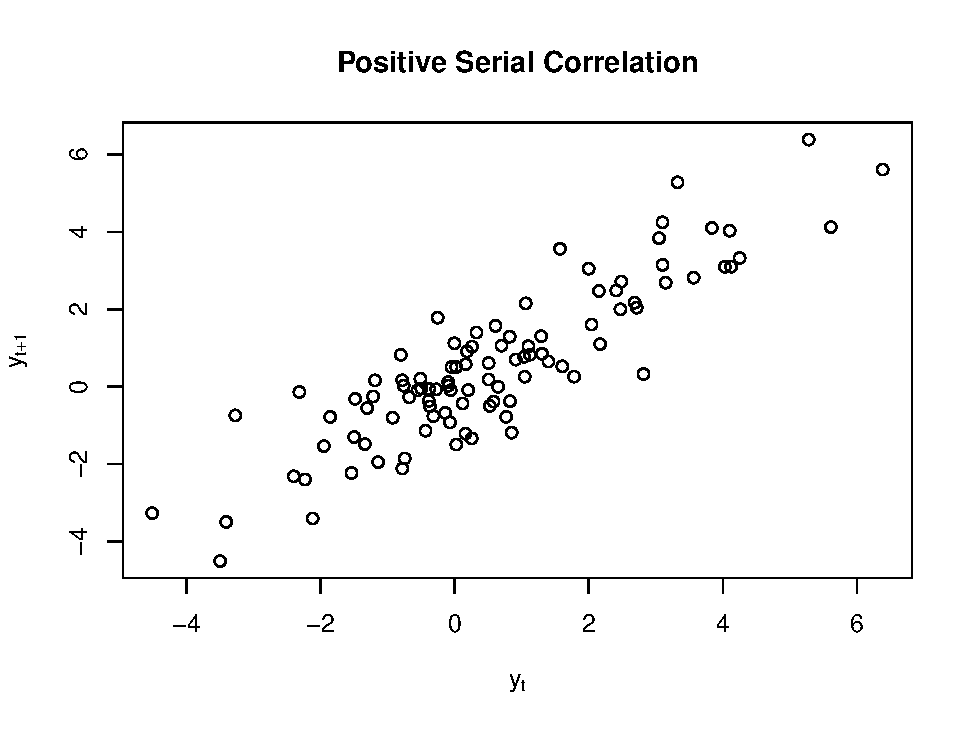
\includegraphics[width=0.8\linewidth]{bookdown-demo_files/figure-latex/ch1-figure2-1} 

}

\caption{Serial Correlation}\label{fig:ch1-figure21}
\end{figure}\begin{figure}

{\centering 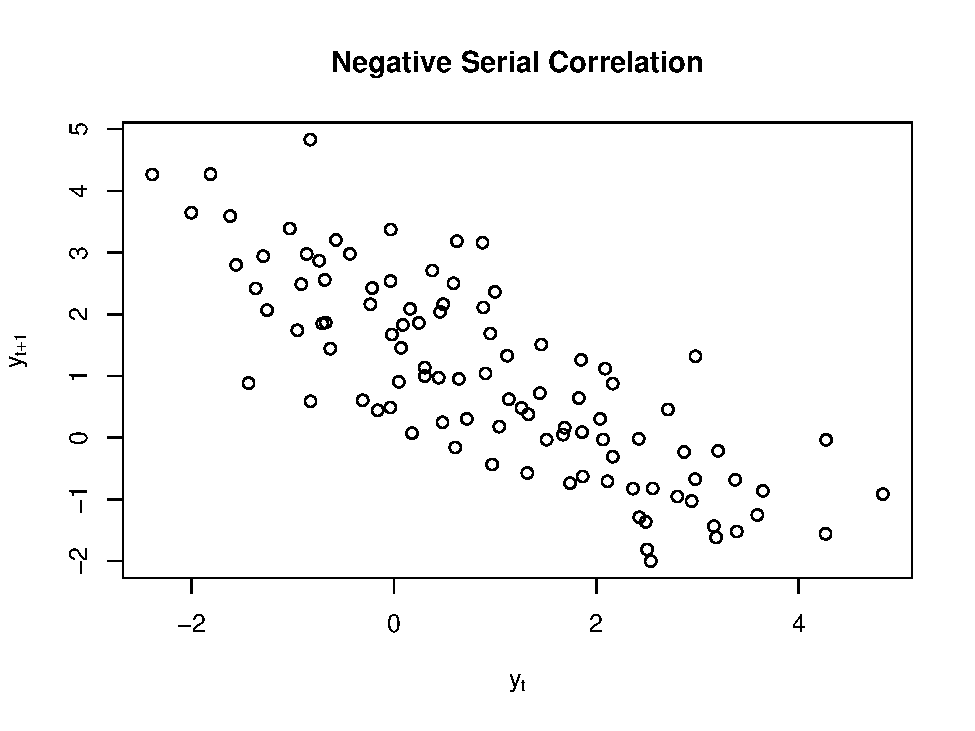
\includegraphics[width=0.8\linewidth]{bookdown-demo_files/figure-latex/ch1-figure2-2} 

}

\caption{Serial Correlation}\label{fig:ch1-figure22}
\end{figure}

\hypertarget{testing-for-serial-correlion}{%
\section{Testing for Serial Correlion}\label{testing-for-serial-correlion}}

We can use a Lagrange-Multiplier (LM) test for detecting serial correlation. This test is also known as \emph{Breuch-Godfrey} test. I will use the linear regression model to explain this test. Consider the following regression model:
\begin{equation}
y_t=\beta_0 + \beta_1 X_{1t}+\epsilon_t
\end{equation}

Consider the following model for serial correlation of order \emph{p} for the error term:
\begin{equation}
\epsilon_t=\rho_1 \epsilon_{t-1}+\rho_2 \epsilon_{t-2}+...+ \rho_p \epsilon_{t-p}+\nu_t
\label{eq:bg}
\end{equation}

Then we are interested in the following test:

\[H_0=\rho_1=\rho_2=...=\rho_p=0 \]
\[H_A = Not \ H_0 \]

To implement this test, we estimate the BG regression model given by:
\begin{equation}
e_t=\alpha_0 + \alpha_1 X_{1t}+ \rho_1 e_{t-1}+\rho_2 e_{t-2}+...+ \rho_p e_{t-p}+\nu_t
\label{eq:bg1}
\end{equation}

where we replacr the error term with the OLS residuals (denoted by \(e\)). The LM test statistic is given by:

\[ LM  = N\times R^2_{BG}  \sim \chi^2_p  \]

If the test statistic value is greater than the critical value then we reject the null hypothesis.

\hypertarget{white-noise-process}{%
\section{White Noise Process}\label{white-noise-process}}

A time series is a \emph{white noise} process is it has zero mean, constant and finite variance, and is serially uncorrelated. Formally, \(y_t\) is a white noise process if:

\begin{enumerate}
\def\labelenumi{\arabic{enumi}.}
\tightlist
\item
  \(E(y_t)=0\)
\item
  \(Var(y_t)=\sigma^2_y\)
\item
  \(Cov(y_t,y_{t-s})= 0 \forall s\neq t\)
\end{enumerate}

We can compress the above definition as: \(y_t\sim WN(0,\sigma^2_y)\).
Often we assume that the unexplained part of a time series follows a white noise process. Formally,

\begin{equation}
Time \ Series \ = \  Explained  \ + \ White \ Noise
\end{equation}

By definition we cannot forecast a white noise process. An important diagnostics of model adequacy is to test whether the estimated residuals are white noise (more on this later).

\hypertarget{important-elements-of-forecasting}{%
\section{Important Elements of Forecasting}\label{important-elements-of-forecasting}}

\BeginKnitrBlock{definition}[Forecast]
\protect\hypertarget{def:d1}{}{\label{def:d1} \iffalse (Forecast) \fi{} }
\EndKnitrBlock{definition}

A \emph{forecast} is an \emph{informed} guess about the unknown future value of a time series of interest. For example, what is the stock price of Facebook next Monday?

There are three possible types of forecasts:

\begin{enumerate}
\def\labelenumi{\arabic{enumi}.}
\tightlist
\item
  \emph{Density Forecast}: we forecast the entire probability distribution of the possible future value of the time series of interest. Hence,
\end{enumerate}

\begin{equation}
F(a)=P[y_{t+1}\leq a]
\end{equation}

give us the probability that the 1-period ahead future value of \(y_{t+1}\) will be less than or equal to \(a\). For example, the future real GDP growth could be normally distributed with a mean of 1.3\% and a standard deviation of 1.83\%. Figure \ref{fig:ch1-figure3} below plots the density forecast for real GDP growth.

\begin{figure}

{\centering 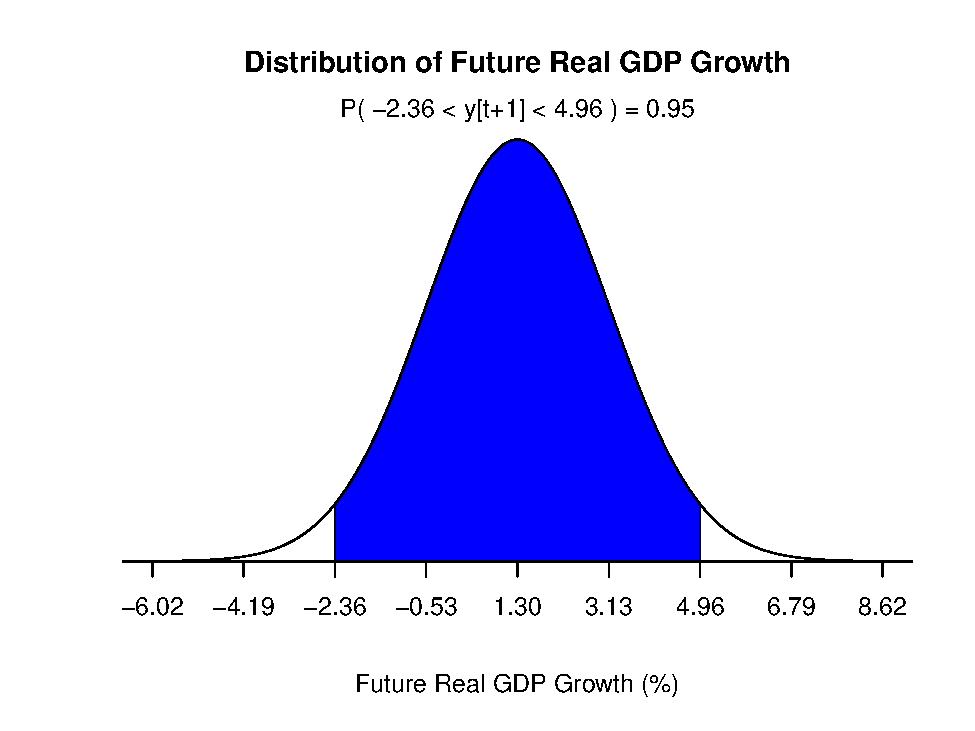
\includegraphics[width=0.8\linewidth]{bookdown-demo_files/figure-latex/ch1-figure3-1} 

}

\caption{Density Forecast for Future Real GDP Growth}\label{fig:ch1-figure3}
\end{figure}

\begin{enumerate}
\def\labelenumi{\arabic{enumi}.}
\setcounter{enumi}{1}
\item
  \emph{Point Forecast}: our forecast at each horizon is a single number. Often we use the expected value or mean as the point forecast. For example, the point forecast for the 1-period ahead real GDP growth can be the mean of the probability distribution of the future real GDP growth:
  \begin{equation}
  f_{t,1}=1.3%
  \end{equation}
\item
  \emph{Interval Forecast}: our forecast at each horizon is a range which is obtained by adding \emph{margin of errors} to the point forecast. With some probability we expect our future value to fall withing this range. For example, the 95\% interval forecast for the next period real GDP growth is (-2.36\%,4.96\%). Hence, with 95\% confidence we expect next period GDP to fall between -2.36\% and 4.96\%.
\end{enumerate}

\BeginKnitrBlock{definition}[Forecast Horizon]
\protect\hypertarget{def:d2}{}{\label{def:d2} \iffalse (Forecast Horizon) \fi{} }
\EndKnitrBlock{definition}

\emph{Forecast Horizon} is the number of periods into the future for which we forecast a time series. We will denote it by \(h\). Hence, for \(h=1\), we are looking at 1-period ahead forecast, for \(h=2\) we are looking at 2-period ahead forecast and so on.

Formally, for a given time series \(y_t\), the h-period ahead unknown value is denoted by \(y_{t+h}\). The forecast of this value is denoted \(f_{t,h}\).

\begin{figure}

{\centering 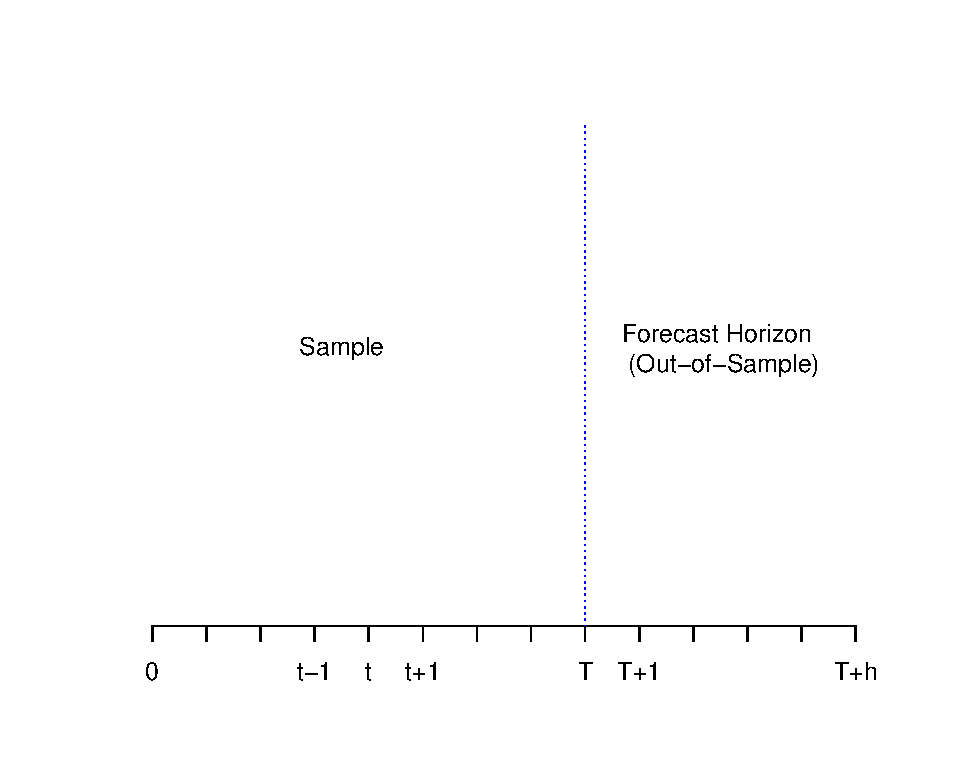
\includegraphics[width=0.8\linewidth]{bookdown-demo_files/figure-latex/ch1-figure4-1} 

}

\caption{Forecast Horizon}\label{fig:ch1-figure4}
\end{figure}

\BeginKnitrBlock{definition}[Forecast Error]
\protect\hypertarget{def:d3}{}{\label{def:d3} \iffalse (Forecast Error) \fi{} }
\EndKnitrBlock{definition}

A \emph{forecast error} is the difference between the realization of the future value and the previously made forecast. Formally, the \(h\)-period ahead forecast error is given by:

\begin{equation}
e_{t,h}=y_{t+h}-f_{t,h}
\end{equation}

Hence, for every horizon, we will have a forecast and a corresponding forecast error. These errors can be negative (indicating over prediction) or positive (indicating under prediction).

\BeginKnitrBlock{definition}[Information Set]
\protect\hypertarget{def:d4}{}{\label{def:d4} \iffalse (Information Set) \fi{} }
\EndKnitrBlock{definition}

Forecasts are based on \emph{information} available at the time of making the forecast. \emph{Information Set} contains all the relevant information about the time series we would like to forecast. We denote the set of information available at time \(T\) by \(\Omega_T\). There are two types of information sets:

\begin{enumerate}
\def\labelenumi{\arabic{enumi}.}
\item
  Univariate Information set: Only includes historical data on the time series of interest:
  \begin{equation}
  \Omega_T=\{y_T, y_{T-1}, y_{T-2}, ...., y_1\}
  \end{equation}
\item
  Multivariate Information set: Includes historical data on the time series of interest as well as any other variable(s) of interest. For example, suppose we have one more variable \(x\) that is relevant for forecasting \(y\). Then:
  \begin{equation}
  \Omega_T=\{y_T, x_T, y_{T-1}, x_{T-1}, y_{T-2},x_{T-2}. ...., y_1, x_1\}
  \end{equation}
\end{enumerate}

\hypertarget{loss-function-and-optimal-forecast}{%
\section{Loss Function and Optimal Forecast}\label{loss-function-and-optimal-forecast}}

Think of a forecast as a solution to an \emph{optimization} problem. When forecasts are wrong, the person making the forecast will suffer some \emph{loss}. This loss will be a function of the magnitude as well as the sign of the \emph{forecast error}. Hence, we can think of an \emph{optimal forecast} as a solution to a minimization problem where the forecaster is minimizing the loss from the forecast error.

\BeginKnitrBlock{definition}[Loss Function]
\protect\hypertarget{def:d5}{}{\label{def:d5} \iffalse (Loss Function) \fi{} }
\EndKnitrBlock{definition}

A \emph{loss} function is a mapping between forecast errors and their associated losses. Formally, we denote the h-period ahead loss function by \(L(e_{t,h})\). For a function to be used as a loss function, three properties must be satisfied:

\begin{enumerate}
\def\labelenumi{\arabic{enumi}.}
\tightlist
\item
  \(L(0)=0\)
\item
  \(\frac{dL}{de}>0\)
\item
  \(L(e)\) is a continuous function.
\end{enumerate}

Two types of loss functions are:

\begin{itemize}
\tightlist
\item
  Symmetric Loss Function: both positive and negative forecast errors lead to same loss. See Figure \ref{fig:ch1-figure5}. A commonly used loss function is \emph{quadratic loss function} given by:
\end{itemize}

\begin{equation}
L(e_{t,h})=e_{t,h}^2 = (y_{t+h}-f{t,h})^2
\end{equation}

\begin{figure}

{\centering 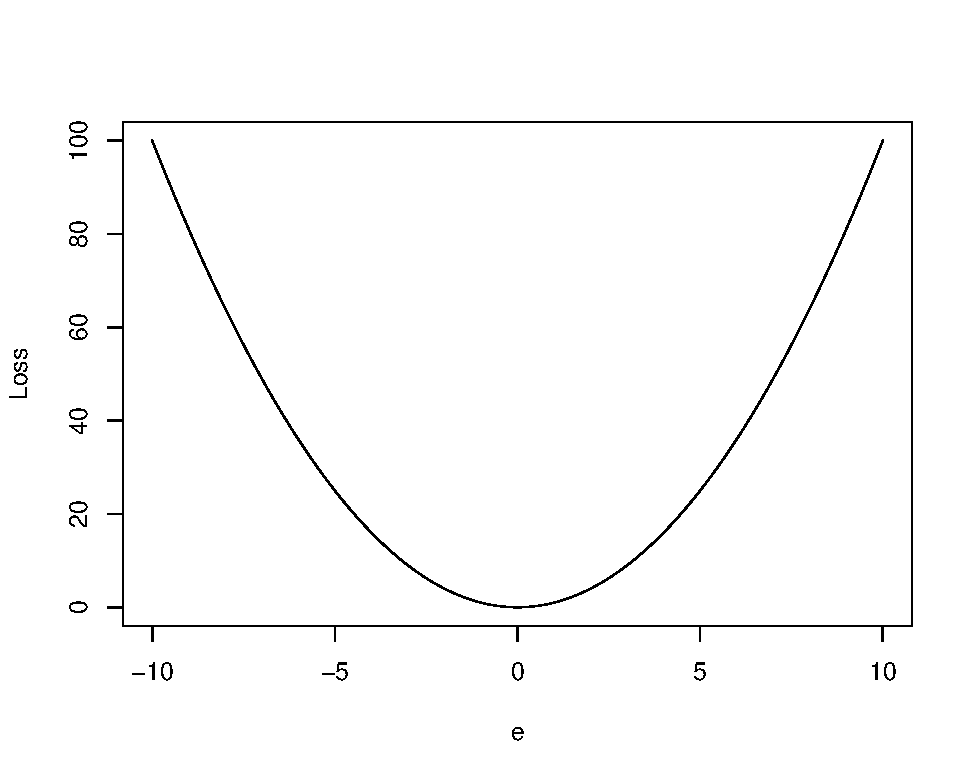
\includegraphics[width=0.8\linewidth]{bookdown-demo_files/figure-latex/ch1-figure5-1} 

}

\caption{Quadratic Loss Functions}\label{fig:ch1-figure5}
\end{figure}

\begin{itemize}
\tightlist
\item
  Asymmetric Loss Function: loss depends on the sign of the forecast error. For example, it could be that positive errors produce greater loss when compared to negative errors. See the function below and Figure \ref{fig:ch1-figure6} that attaches a higher loss to positive errors:
\end{itemize}

\begin{equation}
L(e_{t,h})=e_{t,h}^2+4 \times e_{t,h}
\end{equation}

\begin{figure}

{\centering 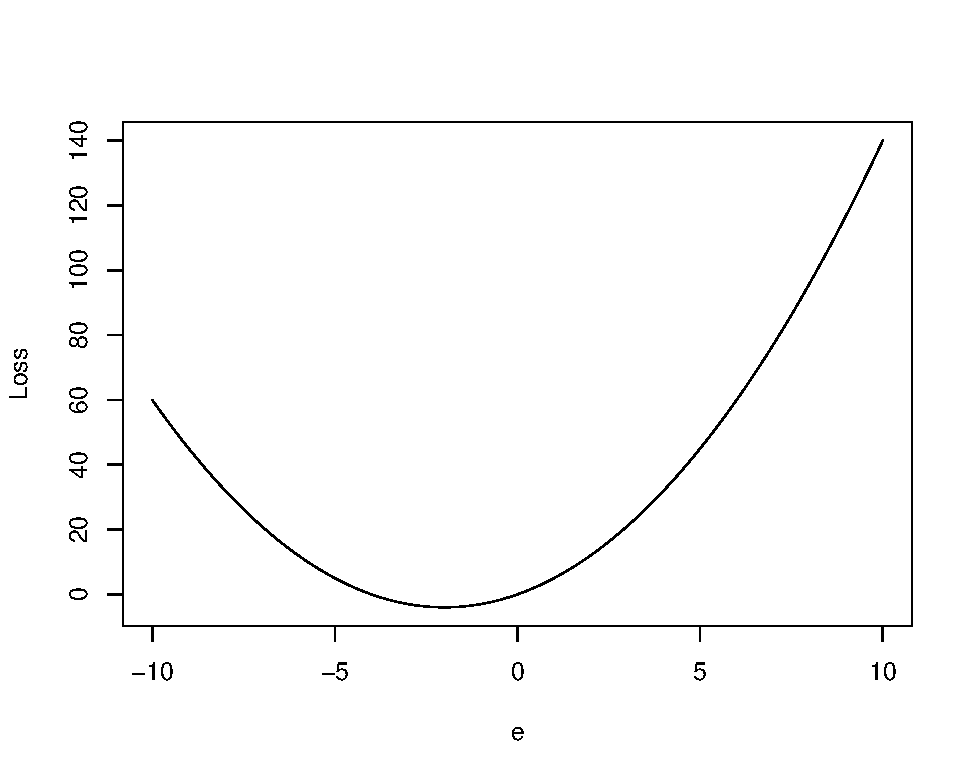
\includegraphics[width=0.8\linewidth]{bookdown-demo_files/figure-latex/ch1-figure6-1} 

}

\caption{Asymmetric Loss Function}\label{fig:ch1-figure6}
\end{figure}

Once we have chosen our loss function, the optimal forecast can be obtained by minimizing the expected loss function.

\BeginKnitrBlock{definition}[Optimal Forecast]
\protect\hypertarget{def:d6}{}{\label{def:d6} \iffalse (Optimal Forecast) \fi{} }
\EndKnitrBlock{definition}

An \emph{optimal forecast} minimizes the expected loss from the forecast, given the information available at the time. Mathematically, we denote it by \(f^*_{t,h}\) and it solves the following minimization problem:
\begin{equation}
min_{f_{t,h}} E(L(e_{t,h})|\Omega_t)
\end{equation}

In theory we can assume any functional form for the loss function and that will lead to a different \emph{optimal forecast}. An important result that follows from a specific functional form is stated as Theorem 1.1.

\BeginKnitrBlock{theorem}
\protect\hypertarget{thm:unnamed-chunk-2}{}{\label{thm:unnamed-chunk-2} }If the loss function is quadtratic then the optimal forecast is the conditional mean of the time series of interest. Formally, if \(L(e_{t,h})=e_{t,h}^2\) then,
\begin{equation}
f^*_{t,h}=E(y_{t+h}|\Omega_t)
\end{equation}
\EndKnitrBlock{theorem}

Note that \(E(e_{t,h}^2)\) is known as \emph{mean squared errors (MSE)}. Hence, the expected loss from a quadratic loss function is the same as the MSE. In this course, we assume that the forecaster faces a quadratic loss function and hence based on Theorem 1.1, we will learn different models for estimating the conditional mean of the future value of the time series of interest, i.e., \(E(y_{t+h}|\Omega_t)\).

\hypertarget{regression-based-forecasting}{%
\chapter{Regression-based Forecasting}\label{regression-based-forecasting}}

One way to compute the conditional expectation is the linear regression model. Here, our information set contains data on all relevant explanatory variables available at the time of forecast, i.e,

\begin{equation}
\Omega_t={X_{1t}, X_{2t},...X_{Kt}}
\end{equation}

Hence, we get the following equality:

\begin{equation}
E(y_t|\Omega_t)=E(y_{t}|X_{1t}, X_{2t}, X_{3t},...,X_{Kt})
\end{equation}

The right hand side of the above equation is the multiple regression model of the form:
\begin{equation}
 y_{t}=\beta_0+\beta_1 X_{1t}+\beta_2 X_{2t}+..+\beta_K X_{Kt}+\epsilon_t
 \end{equation}

We can easily estimate the above model using Ordinary Least Squares (OLS) and compute the \emph{predicted value} of \(y\):
\begin{equation}
    \widehat{y}_t = \widehat{\beta_0} +\widehat{\beta_1} X_{1t} +\widehat{\beta_2} X_{2t}+...+ \widehat{\beta_k} X_{Kt}
  \end{equation}

The above equation can be used to compute the optimal forecast. Suppose, we are interested in computed the \(h\) period ahead forecast for \(y\). Then, using the above equation we get:
\begin{equation}
        \widehat{y}_{t+h} =  \widehat{\beta_0} +\widehat{\beta_1} X_{1t+h} +\widehat{\beta_2} X_{2t+h}+...+ \widehat{\beta_k} X_{Kt+h}
    \end{equation}

\hypertarget{scenario-analysis-and-conditional-forecasts}{%
\section{Scenario Analysis and Conditional Forecasts}\label{scenario-analysis-and-conditional-forecasts}}

One way to use a regression model to produce forecasts is called
\emph{scenario analysis} where we produce a different forecast for the dependent under each possible scenario about the future values of the independent variables. For example, what will be the forecast for inflation if the Federal Reserve Bank raises the interest rate? Would our forecast differ depending on the size of the increase in the interest rate?

\hypertarget{unconditional-forecasts}{%
\section{Unconditional Forecasts}\label{unconditional-forecasts}}

An alternative is to separately forecast each independent variable and then compute the forecast for the dependent variable. Yet another alternative is to use lagged variables as independent variables. Depending on the number of lags, we can forecast that much ahead into future (see Distributed Lag Section for details).

\hypertarget{some-practical-issues}{%
\section{Some practical issues}\label{some-practical-issues}}

\begin{enumerate}
\def\labelenumi{\arabic{enumi}.}
\item
  To forecast the dependent variable we first need to compute a forecast for the independent variable. Errors in this step induce errors later.
\item
  \emph{Spurious regression}: It is quite possible to find a strong linear relationship between two completely unrelated variables over time if they share a common time trend.
\item
  \emph{Model Uncertainty}: We do not know the true functional form for the regression model and hence our estimated model is only a proxy for the true model.
\item
  \emph{Parameter Uncertainty}: This kind of forecast uses regression coefficients that are computed using a fixed sample. Over time with new data, there will be changes in these coefficients.
\end{enumerate}

\hypertarget{distributed-lag-regression-models}{%
\section{Distributed Lag Regression Models}\label{distributed-lag-regression-models}}

Consider the following simple regression model:

\begin{equation}
y_t= \beta_0 +\beta_1 x_t + \epsilon_t
\end{equation}

Here, if want to forecast \(y_{t+1}\) then we must either consider different scenarios for \(x_{t+1}\) or independently forecast \(x_{t+1}\) first, and then use it to compute forecast for \(y_{t+1}\). An alternative is to estimate the following lagged regression model:

\begin{equation}
y_t= \beta_0 +\beta_1 x_{t-1} + \epsilon_t
\end{equation}

Note that by estimating the above model we get the following predicted value equation for \(t+1\):

\begin{equation}
\widehat{y_{t+1}}=\widehat{\beta_0}+\widehat{\beta_1}x_{t}
\end{equation}

Hence, we can easily produce 1-period ahead forecast from this model. In order to produce forecast farther into future we would need to add more lags of the independent variable to the model. A generalized model of this kind is called \emph{distributed lag model} and is given by:
\begin{equation}
y_t= \beta_0 +\sum_{s=1}^p\beta_s x_{t-s} + \epsilon_t
\end{equation}

The number of lags to include can be determined using some kind of goodness of fit measure.

\hypertarget{dynamic-effect-of-x-on-y}{%
\subsection{Dynamic Effect of X on Y}\label{dynamic-effect-of-x-on-y}}

A very useful benefit of estimating a distributed lag model is that it allows us to measure how changes in \(x\) in the current period can impact the dependent variable over time. Consider a simple distributed lag model with two lags:
\begin{equation}
y_t=\beta_0 + \beta_1 x_{t-1} + \beta_2 x_{t-2} +\epsilon_t
\end{equation}

In this model the lag structure implies that any change in \(x\) will persist for two periods in terms of its effect on \(y\). In fact we now have to consider the \emph{dynamic} effect of \(x\) on \(y\). Formally, there are two types of effects:

\begin{enumerate}
\def\labelenumi{\arabic{enumi}.}
\tightlist
\item
  \emph{dynamic effect} of \(x\) on \(y\) given by:
  \[\frac{\partial y_{t+s}}{\partial x_t} \quad s=0,1,2,...\]
\end{enumerate}

In our example, the sequence of dynamic effects are:
\begin{equation}
\frac{\partial y_{t}}{\partial x_t}  =0; \ \frac{\partial y_{t+1}}{\partial x_t}=\beta_1; \ \frac{\partial y_{t+2}}{\partial x_t}=\beta_2; \ \frac{\partial y_{t+s}}{\partial x_t}=0 \ \forall \ s>2 
\end{equation}

\begin{enumerate}
\def\labelenumi{\arabic{enumi}.}
\setcounter{enumi}{1}
\tightlist
\item
  \emph{long run effect} of \(x\) on \(y\) given by:
  \begin{equation}
  \sum_{s=0}^p\frac{\partial y_{t+s}}{\partial x_t}   
  \end{equation}
\end{enumerate}

In our example, the long run effect is:

\[\beta_1+\beta_2\]

\hypertarget{model-selection-criterion}{%
\subsection{Model Selection Criterion}\label{model-selection-criterion}}

Most often we compare models that have different number of independent variables. For example, in our application, in order to select the number of lags for output and capital stock, we will essentially compare models with different number of independent variables. In such cases we must account for the trade-off between goodness of fit and degrees of freedom. Increasing the number of independent variables will:

\begin{enumerate}
\def\labelenumi{\arabic{enumi}.}
\item
  lower the MSE and hence leads to better fit.
\item
  lowers the degrees of freedom
\end{enumerate}

Two commonly used measures based on MSE incorporate this trade-off:

\begin{enumerate}
\def\labelenumi{\arabic{enumi}.}
\tightlist
\item
  Akaike Information Criterion (AIC):
  \[ AIC= MSE \times e^{\frac{2k}{T}} \]
\end{enumerate}

where \(k\) is the number of estimated parameters, \(T\) is the sample size. Then, \(K/T\) is the number of parameters estimated per observation and \(e^{\frac{2k}{T}}\) is the \emph{penalty factor} imposed on adding more variables to the model. As we increase \(k\), this penalty factor will increase exponentially for a given value of \(T\).

\begin{enumerate}
\def\labelenumi{\arabic{enumi}.}
\setcounter{enumi}{1}
\tightlist
\item
  Bayesian Information Criterion (BIC):
\end{enumerate}

\[ BIC= MSE \times T^{\frac{k}{T}} \]

Lower values of either AIC or BIC indicates greater accuracy. So we select a model with lower value of either of these two criteria. Note that the penalty imposed by BIC is harsher and hence it will typically select a more parsimonious model (Figure \ref{fig:ch2-figure1}).

\begin{figure}

{\centering 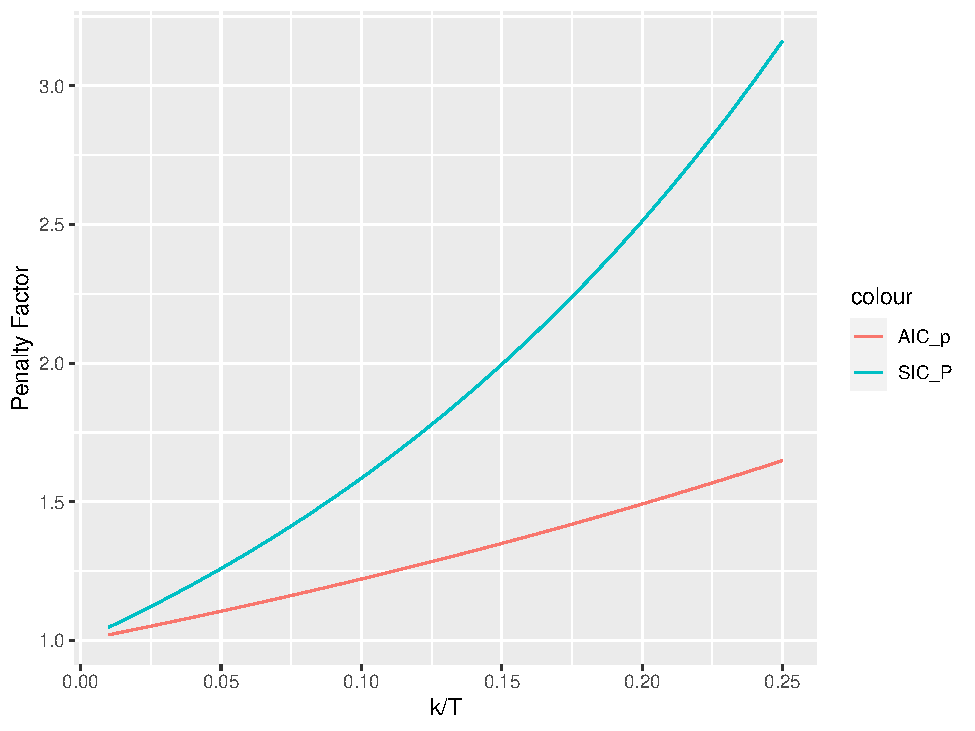
\includegraphics[width=0.8\linewidth]{bookdown-demo_files/figure-latex/ch2-figure1-1} 

}

\caption{Penalty Factor of AIC and BIC}\label{fig:ch2-figure1}
\end{figure}

\hypertarget{application-a-model-of-investment-expenditure}{%
\section{Application: A Model of Investment Expenditure}\label{application-a-model-of-investment-expenditure}}

\hypertarget{a-multiple-regression-model-of-invesment-expenditure}{%
\subsection{A Multiple Regression Model of Invesment Expenditure}\label{a-multiple-regression-model-of-invesment-expenditure}}

Suppose have annual data on private investment, private sector output, and capital stock. Our model specification is given by:
\begin{equation}
y_t= \beta_0 + \beta_1 x_{1t}+ \beta_2 x_{2t}+\epsilon_t
\end{equation}

We can estimate the above model using OLS and then conduct scenario-based forecasting. For ease of interpretation, we will convert all variables in natural logarithms.

Table \ref{tab:ch2-table1} below presents the estimated coefficients of our regression model. Higher output and capital stock leads to greater investment expenditure.

\begin{table}[t]

\caption{\label{tab:ch2-table1}A Multiple Regression Model of Investment Expenditure}
\centering
\begin{tabular}{lcccc}
\toprule
  & Estimated Coefficients & Std. Error & t-ratio & p-value\\
\midrule
(Intercept) & -4.8421855 & 0.9623332 & -5.031714 & 0.0000044\\
x1 & 0.9987751 & 0.2418282 & 4.130102 & 0.0001104\\
x2 & 0.4204833 & 0.3643054 & 1.154205 & 0.2528456\\
\bottomrule
\end{tabular}
\end{table}

Next, we forecast of investment expenditure under three different scenarios:

\begin{enumerate}
\def\labelenumi{\arabic{enumi}.}
\item
  For next 3 years, both output and capital stock remain at the average of last 3 years.
\item
  For next 3 years, both output and capital stock remain at 1\% above the average of last 3 years.
\item
  For next 3 years, both output and capital stock remain at 1\% below the average of last 3 years.
\end{enumerate}

Figure \ref{fig:ch2-figure2} below present our investment expenditure outlook under these 3 scenarios.

\begin{verbatim}
## Error in forecast(fit, newdata = newdata, level = 95): unused arguments (newdata = newdata, level = 95)
\end{verbatim}

\begin{verbatim}
## Error in forecast(fit, newdata = newdata, level = 95): unused arguments (newdata = newdata, level = 95)
\end{verbatim}

\begin{verbatim}
## Error in forecast(fit, newdata = newdata, level = 95): unused arguments (newdata = newdata, level = 95)
\end{verbatim}

\begin{verbatim}
## Error in plot(s1, include = 25, main = "Scenario 1"): object 's1' not found
\end{verbatim}

\begin{verbatim}
## Error in plot(s2, include = 25, main = "Scenario 2"): object 's2' not found
\end{verbatim}

\begin{verbatim}
## Error in plot(s3, include = 25, main = "Scenario 3"): object 's3' not found
\end{verbatim}

\hypertarget{a-distributed-lag-model-of-investment-expenditure}{%
\subsection{A Distributed Lag Model of Investment Expenditure}\label{a-distributed-lag-model-of-investment-expenditure}}

In this application we will estimate a distributed lag model for investment expenditure. The idea here is that it takes time for investment to respond to output and capital stock changes. The model specification we want to estimate is:

\begin{equation}
y_t= \beta_0 + \sum_{i=1}^p\beta_i x_{1t-i}+\sum_{i=1}^p\alpha_i x_{2t-i}+\epsilon_t
\end{equation}

where \(y\) denotes real investment expenditure of the private sector, \(x_1\) denotes output of the private sector, and \(x_2\) denotes capital stock of the private sector.

We estimate our model by first selecting the optimal lag order for each independent variable, and selecting the one with lowest value for AIC/BIC. From @\ref(tab:ch2-table2) we find that the lowest BIC occurs at lag=2. Hence, we estimate a model with two lags for each independent variable in our model.

\begin{verbatim}
## Error in library(dynlm): there is no package called 'dynlm'
\end{verbatim}

\begin{verbatim}
## Error in dynlm(formula = y ~ L(x1, 1:k) + L(x2, 1:k)): could not find function "dynlm"
\end{verbatim}

\begin{table}[t]

\caption{\label{tab:ch2-table2}Optimal Order of the lags}
\centering
\begin{tabular}{ccc}
\toprule
Lag & AIC & BIC\\
\midrule
1 & 0 & 0\\
2 & 0 & 0\\
3 & 0 & 0\\
4 & 0 & 0\\
\bottomrule
\end{tabular}
\end{table}

Hence, our final model is given by:
\begin{equation}
y_t= \beta_0 + \sum_{i=1}^2\beta_i x_{1t-i}+\sum_{i=1}^2\alpha_i x_{2t-i}
\end{equation}

The results of our estimation are presented below in Table \ref{tab:ch2-table3}

\begin{verbatim}
## Error in dynlm(formula = y ~ L(x1, 1:2) + L(x2, 1:2)): could not find function "dynlm"
\end{verbatim}

\begin{verbatim}
## Error in summary(final): object 'final' not found
\end{verbatim}

\begin{enumerate}
\def\labelenumi{\arabic{enumi}.}
\item
  Using our estimated model we can easily compute the dynamic effect as well as the long run effect of each independent variable on the dependent variable.
\item
  Given the lag structure of our estimated model, we can also produce forecasts for \(y_{t+1}\) by computing the following equation:
\end{enumerate}

\begin{equation}
f_{t,1}=\widehat{y_{t+1}}=\hat{\beta_0}+\hat{\beta_1}x_{1t} + \hat{\beta_2}x_{1t-1}+ \hat{\alpha_1}x_{2t}+\hat{\alpha_2}x_{2t-1}
\end{equation}

\hypertarget{components-of-a-time-series}{%
\chapter{Components of a Time Series}\label{components-of-a-time-series}}

A given time series can have four possible components:

\begin{enumerate}
\def\labelenumi{\arabic{enumi}.}
\item
  Trend: denoted by \(B_t\) captures the long run behavior of the time series of interest.
\item
  Season: denoted by \(S_t\) are \emph{periodic} fluctuations over \emph{seasons}. The period of the season is fixed and known. For example, rise in non-durable sales during Christmas.
\item
  Cycle: denoted by \(C_t\) are \emph{non-periodic} are fluctuations in that they occur regularly but over periods that are not fixed in duration.
\item
  Irregular: denoted by \(\epsilon_t\) are random fluctuations, typically modeled as a white noise process.
\end{enumerate}

\hypertarget{decomposing-a-time-series}{%
\section{Decomposing a time series}\label{decomposing-a-time-series}}

We can decompose any given time series into its components. There are two ways to accomplish this:

\begin{enumerate}
\def\labelenumi{\arabic{enumi}.}
\item
  Additive Decomposition: Here it is assumed that all four components are added to obtain the underlying timer series:
  \begin{equation}
  y_t= B_t+S_t+C_t +\epsilon_t
  \end{equation}
\item
  Multiplicative Decomposition: Here it is assumed that all four components are multiplied to obtain the underlying timer series:
  \begin{equation}
  y_t= B_t \times S_t \times C_t \times \epsilon_t
  \end{equation}
\end{enumerate}

Note that using properties of logarithms, multiplicative decomposition is the same as additive decomposition in log terms:
\begin{equation}
log(y_t)= log(B_t) + log(S_t) + log(C_t) + log(\epsilon_t)
\end{equation}

Most statistical software can implement these decomposition using data on a time series variable as input. Typically they combine cyclical component with irregular component and provide a three-way decomposition. In Figure \ref{fig:ch3-figure1} I use R to decompose real GDP for the US into its components.

\begin{figure}

{\centering 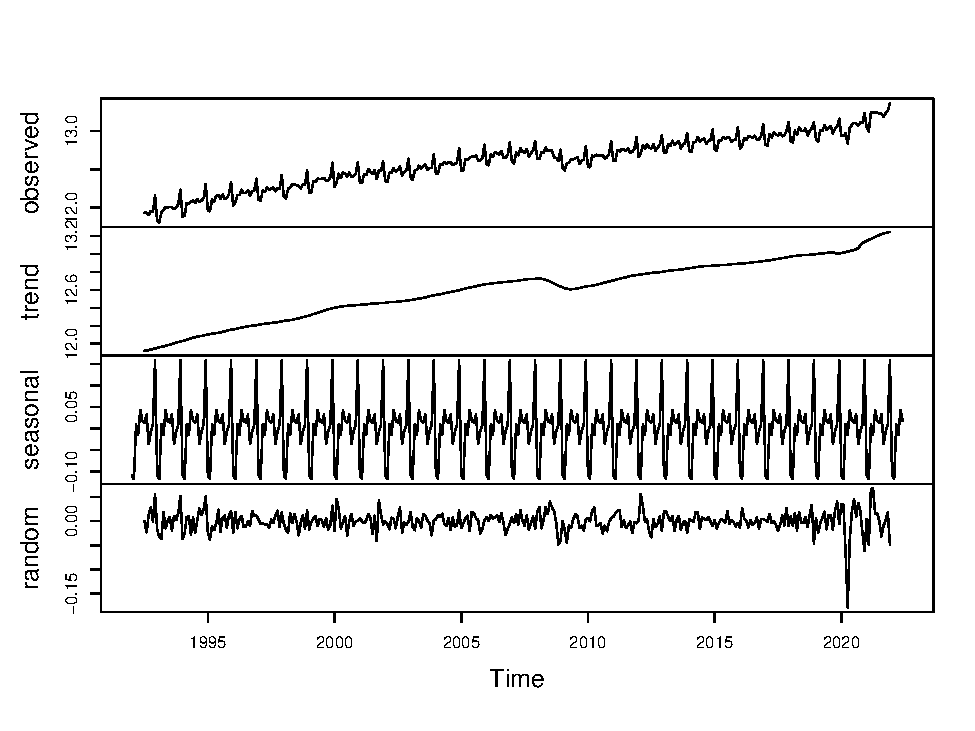
\includegraphics[width=0.8\linewidth]{bookdown-demo_files/figure-latex/ch3-figure1-1} 

}

\caption{Additive Decomposition of Retail Sales}\label{fig:ch3-figure1}
\end{figure}

\hypertarget{uses-of-decomposition-of-a-time-series}{%
\section{Uses of Decomposition of a time series}\label{uses-of-decomposition-of-a-time-series}}

The usefulness of decomposing a time series depends on our objective.

\begin{enumerate}
\def\labelenumi{\arabic{enumi}.}
\item
  It may be of interest to study each component separately or to simply improve our understanding of the temporal dynamics of a time series of interest. Decomposing it into different components is the first step towards achieving that goal.
\item
  We can also use the decomposition to filter out components that we are not interested in studying. If for example we are only interested in modeling the cyclical component of the time series, then we can assume some kind decomposition, additive or multiplicative, and filter out the trend and seasonal component. For example, assuming additive decomposition, the filtered time series is given by:
  \begin{equation}
  Filtered \ y_t= y_t-B_t-S_t
  \end{equation}
\end{enumerate}

We can then proceed to model the cyclical component using the filtered data.

\hypertarget{smoothing-methods}{%
\chapter{Smoothing Methods}\label{smoothing-methods}}

One way to approach forecasting is to \emph{average} out the fluctuations in the underlying time series to produce a \emph{smoothed} data which can be extrapolated to produce forecasts. These smoothing methods are essentially \emph{model-free} and may not even produce \emph{optimal forecasts}. Depending on the method used one can accommodate seasonal as well as trend components of the underlying time series.

\hypertarget{moving-average-method}{%
\section{Moving Average Method}\label{moving-average-method}}

We compute an average of most recent data values for the time series and use it as a forecast for the next period.

An important parameter is the \emph{window} over which we take the average. Let us denote this window by \(m\), then:
\begin{equation}
    y^s_{t+1}=\frac{\sum \limits_{i=t-m+1}^{t}{y_i}}{m}
    \end{equation}

A larger value of \(m\) produces greater smoothing and most software have a default value of this parameter which can be changed if needed.

\hypertarget{simple-exponential-smoothing}{%
\section{Simple Exponential Smoothing}\label{simple-exponential-smoothing}}

In the moving average method, all observations received same weight. However, it is reasonable to argue that more recent observations may have a greater influence than those in the remote past. In this method, the weight attached to past observations exponentially decay over time. Here is the algorithm for computing the smoothed data and its forecast:

\begin{enumerate}
\def\labelenumi{\arabic{enumi}.}
\item
  Initialize at t=1:
  \[y_1^s=y_1\]
\item
  Update:
  \[y_{t}^{s}= \alpha y_t + (1-\alpha)y_{t-1}^{s}  \quad for \ t=2,3,...T\]
\end{enumerate}

3: h-period ahead forecast:
\[f_{T,h}= y_T^s\]

Here the h-period ahead forecast is:

\emph{Exercise: Can you show that \(y_{t}^{s}\) is a is the weighted moving average of all past observations? Use backward substitution method.}

Here \(\alpha \in (0,1)\) is the smoothing parameter, with smaller value indicating greater smoothing.

\hypertarget{holt-winters-smoothing}{%
\section{Holt-Winters Smoothing}\label{holt-winters-smoothing}}

We add trend component to the simple exponential smoothing. In step 2 the equation we use to update the smoothed data is given by:

\begin{align}
    y_{t}^{s}= \alpha y_t + (1-\alpha)(y_{t-1}^{s}+B_{t-1}) \\ \nonumber
    B_t = \beta (y_t^s -y_{t-1}^s) + (1-\beta) B_{t-1}
 \end{align}

We now have an additional parameter \(\beta\) that is the trend parameter. Here the h-period ahead forecast is:

\begin{align}
  f_{T,h} = y_T^s + h\times B_T
  \end{align}

\hypertarget{holt-winters-smoothing-with-seasonality}{%
\section{Holt-Winters Smoothing with Seasonality}\label{holt-winters-smoothing-with-seasonality}}

We now add seasonal component along with trend. Assuming multiplicative seasonality with period \(n\):

\begin{align}
    y_{t}^{s}= \alpha \frac{y_t}{S_{t-n}} + (1-\alpha)(y_{t-1}^{s}+B_{t-1})\\
    B_t = \beta (y_t^s -y_{t-1}^s) + (1-\beta) B_{t-1}\\
    S_t = \gamma\frac{y_t}{y_t^s}+(1-\gamma)S_{t-n}
  \end{align}

The h-period ahead forecast is given by:

\begin{equation}
    f_{T,h}= (y_T^s + h\times B_T) \times S_{T+h-n}
   \end{equation}

\hypertarget{application}{%
\section{Application}\label{application}}

We use R to implement a 12-period ahead forecast for new housing starts for the U.S. The data is at monthly frequency from Jan 1959 through March 2019. The resulting forecasts are plotted in Figure \ref{fig:ch4-figure1}.

\begin{verbatim}
## Error in forecast(s_exp1, h = 12): unused argument (h = 12)
\end{verbatim}

\begin{verbatim}
## Error in forecast(s_exp2, h = 12): unused argument (h = 12)
\end{verbatim}

\begin{verbatim}
## Error in forecast(s_exp3, h = 12): unused argument (h = 12)
\end{verbatim}

\begin{verbatim}
## Error in plot(f_exp1, include = 24, main = "Simple Exponential Smoothing"): object 'f_exp1' not found
\end{verbatim}

\begin{verbatim}
## Error in plot(f_exp2, include = 24, main = "Holt-Winters with Trend"): object 'f_exp2' not found
\end{verbatim}

\begin{verbatim}
## Error in plot(f_exp3, include = 24, main = "Hold-Winters with Trend and Season"): object 'f_exp3' not found
\end{verbatim}

\hypertarget{modeling-trend-and-seasonal-components}{%
\chapter{Modeling Trend and Seasonal Components}\label{modeling-trend-and-seasonal-components}}

\hypertarget{trend-estimation}{%
\section{Trend Estimation}\label{trend-estimation}}

An important component of a time series is \emph{trend} that captures the long run evolution of the variable of interest. There are two types of trends:

\begin{enumerate}
\def\labelenumi{\arabic{enumi}.}
\item
  Deterministic Trend: the underlying trend component is a \emph{known} function of time with \emph{unknown} parameters.
\item
  Stochastic Trend: the trend component is random.
\end{enumerate}

In this note we will focus on estimating and forecasting deterministic trend models. We will come back to stochastic trend later when we talk about stationarity property of a time series.

\hypertarget{parametrizing-a-deterministic-trend}{%
\subsection{Parametrizing a deterministic trend}\label{parametrizing-a-deterministic-trend}}

Whether or not there is deterministic trend in the data can be typically gleaned by simply plotting the time series over time. For example, Figure @ref(fig: ch5-figure1) below plots real GDP for the US at quarterly frequency. We can observe a positive time trend with real GDP increasing with time. In this section we will learn to \emph{fit} a function that captures this relationship accurately.

\begin{figure}

{\centering 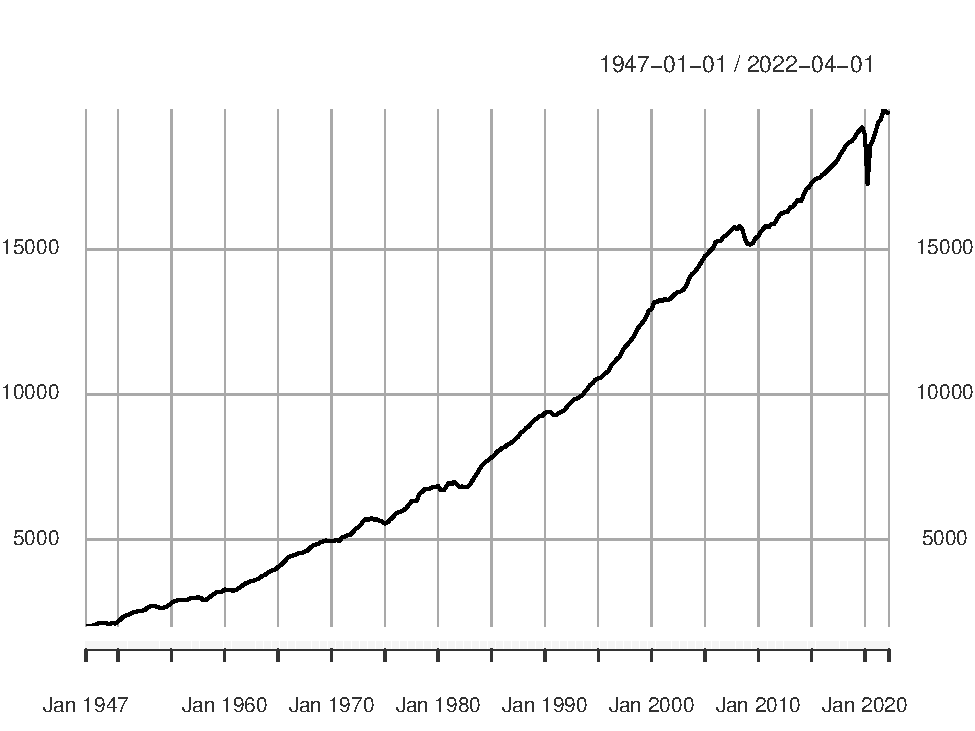
\includegraphics[width=0.8\linewidth]{bookdown-demo_files/figure-latex/ch5-figure1-1} 

}

\caption{Real GDP (2012 Chained Billions of Dollars)}\label{fig:ch5-figure1}
\end{figure}

\emph{Note: The variable time is denoted by \(t\) and it is artificially created to take value of 1 for the first period, 2 for the second period and so on.}

There are two commonly used functional forms for capturing a deterministic trend:

\begin{enumerate}
\def\labelenumi{\arabic{enumi}.}
\tightlist
\item
  Polynomial Trend: We fit a polynomial of appropriate order to capture the time trend. For example,
  A. Linear trend:
  \begin{equation}
  y_t=\beta_0 +\beta_1 t +\epsilon_t
  \end{equation}
\end{enumerate}

B. Quadratic trend:
\begin{equation}
y_t=\beta_0 +\beta_1 t + \beta_2 t^2 +\epsilon_t
\end{equation}

In general, we can fit a polynomial of order \(q\):
\begin{equation}
y_t=\beta_0 + \sum_{i=1}^q \beta_i t^i +\epsilon_t
\end{equation}

We can estimate this model using the OLS. One of the key component here is to determine the \emph{right} order of the polynomial. We can begin with a large enough number for \(q\) and then select the appropriate order using AIC or BIC criterion.

\begin{enumerate}
\def\labelenumi{\arabic{enumi}.}
\setcounter{enumi}{1}
\tightlist
\item
  Exponential or log-linear trend: In some cases we may want to use an exponential trend or equivalently a log-linear trend.
  \begin{align}
  y_t=e^{(\beta_0 +\beta_1 t +\epsilon_t)}\\
  equivalently\\
  log(y_t)=\beta_0 +\beta_1 t +\epsilon_t
  \end{align}
\end{enumerate}

Again we can estimate the above model using OLS.

\hypertarget{uses-of-the-deterministic-trend-model}{%
\subsection{Uses of the Deterministic Trend Model}\label{uses-of-the-deterministic-trend-model}}

Once we have finalized our deterministic trend model i.e., either a polynomial of a specific order or log-liner trend, we can use the estimated model for the following two purposes:

\begin{enumerate}
\def\labelenumi{\arabic{enumi}.}
\item
  Detrending our data: Suppose we would like to eliminate trend from our data. The residual from our final trend model is the \emph{detrended} time series.
\item
  Forecasting: We can also forecast our time series based on the estimated trend. For example, suppose our final model is a quadratic trend. The predicted value is given by:
\end{enumerate}

\begin{equation}
\widehat{y_t}=\widehat{\beta_0}+\widehat{\beta_1} t + \widehat{\beta_2} t^2
\end{equation}

Then, the 1-period ahead forecast for \(y_{t+1}\) can be obtained by solving:
\begin{equation}
\widehat{y_{t+1}}=\widehat{\beta_0}+\widehat{\beta_1} (t+1) + \widehat{\beta_2} (t+1)^2
\end{equation}

\hypertarget{application-estimating-a-polynomial-trend-for-u.s.-real-gdp}{%
\subsection{Application: Estimating a polynomial trend for U.S. Real GDP}\label{application-estimating-a-polynomial-trend-for-u.s.-real-gdp}}

We will now fit a polynomial trend to the US real GDP data that was presented in Figure \ref{fig:figure10}. We first estimate polynomials of different orders and select the optimal order determined by the lowest possible AIC/BIC. Table \ref{tab:ch5-table1}. shows these statistics for up to 4th order polynomial. We find that the lowest value occur at \(q=4\).

\begin{table}[t]

\caption{\label{tab:ch5-table1}Optimal Order of the Polynomial}
\centering
\begin{tabular}{ccc}
\toprule
order & AIC & BIC\\
\midrule
1 & 4792.049 & 4803.048\\
2 & 4190.018 & 4204.684\\
3 & 4158.636 & 4176.968\\
4 & 4070.138 & 4092.136\\
\bottomrule
\end{tabular}
\end{table}

Hence, our final trend model is:

\begin{equation}
y_t=\beta_0 +\beta_1 t + \beta_2 t^2 + \beta_3 t^3 + \beta_4 t^4 +\epsilon_t
\end{equation}

The estimated trend model is presented in Table \ref{tab:ch5-table2}.

\begin{table}[t]

\caption{\label{tab:ch5-table2}Regression Results}
\centering
\begin{tabular}{lcccc}
\toprule
  & Estimate & Std. Error & t value & Pr(>|t|)\\
\midrule
(Intercept) & 1752.959 & 82.098 & 21.352 & 0\\
trend & 40.238 & 3.908 & 10.296 & 0\\
I(trend\textasciicircum{}2) & -0.286 & 0.055 & -5.236 & 0\\
I(trend\textasciicircum{}3) & 0.003 & 0.000 & 9.281 & 0\\
I(trend\textasciicircum{}4) & 0.000 & 0.000 & -10.219 & 0\\
\bottomrule
\end{tabular}
\end{table}

Using the estimated model, we can compute the detrended data as the residual and also forecast \(y_t\). Figure \ref{fig:ch5-figure2} below plots the detrended real GDP obtained as a residual from our trend model.

\begin{figure}

{\centering 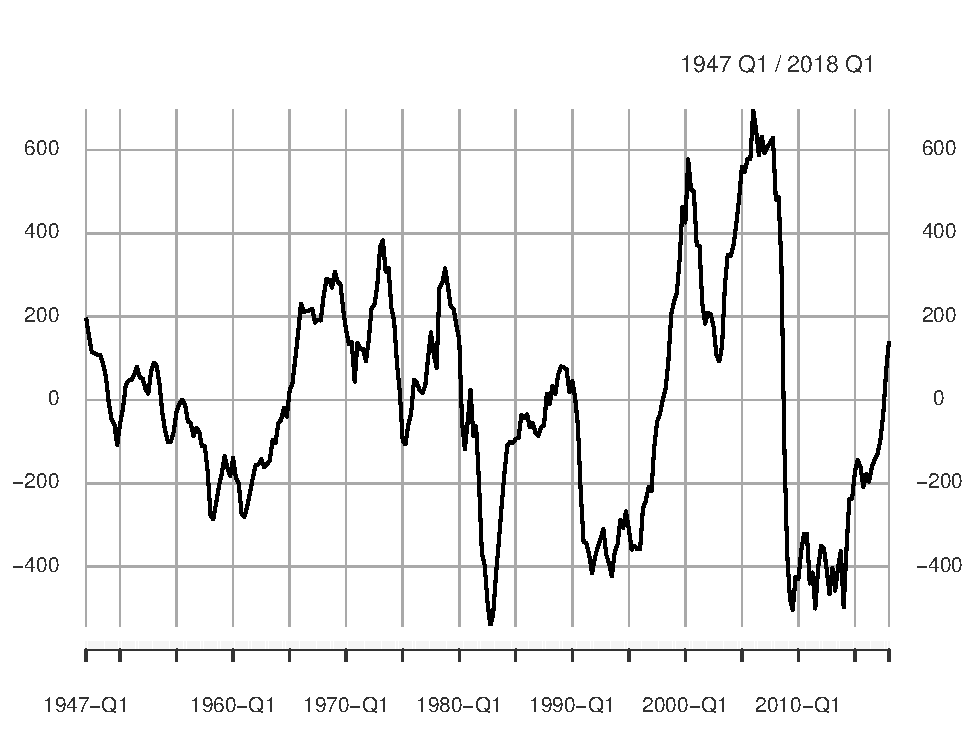
\includegraphics[width=0.8\linewidth]{bookdown-demo_files/figure-latex/ch5-figure2-1} 

}

\caption{Detrended Real GDP}\label{fig:ch5-figure2}
\end{figure}

Figure \ref{fig:ch5-figure3} shows the forecast of real GDP for next 8 quarters along with the 95\% confidence bands.

\begin{verbatim}
## Error in forecast(fit, h = 8): unused argument (h = 8)
\end{verbatim}

\begin{verbatim}
## Error in plot(fcast, include = 24, main = ""): object 'fcast' not found
\end{verbatim}

\hypertarget{seasonal-model}{%
\section{Seasonal Model}\label{seasonal-model}}

We now focus on the \emph{seasonal} component of a time series, i.e., that is periodic fluctuations that repeat themselves every season. For example, increase in ice cream sales during summer season. Just like trend component, such seasonal pattern could be \emph{deterministic} or \emph{stochastic}. In this chapter we will focus on estimating deterministic seasonal component.

In Figure \ref{fig:ch5-figure4} we plot housing starts in the U.S. The data is at monthly frequency and we can see a clear seasonal pattern. Housing starts seem to increase in spring and summer months. This is followed by a decline in fall and winter months.

\begin{figure}

{\centering 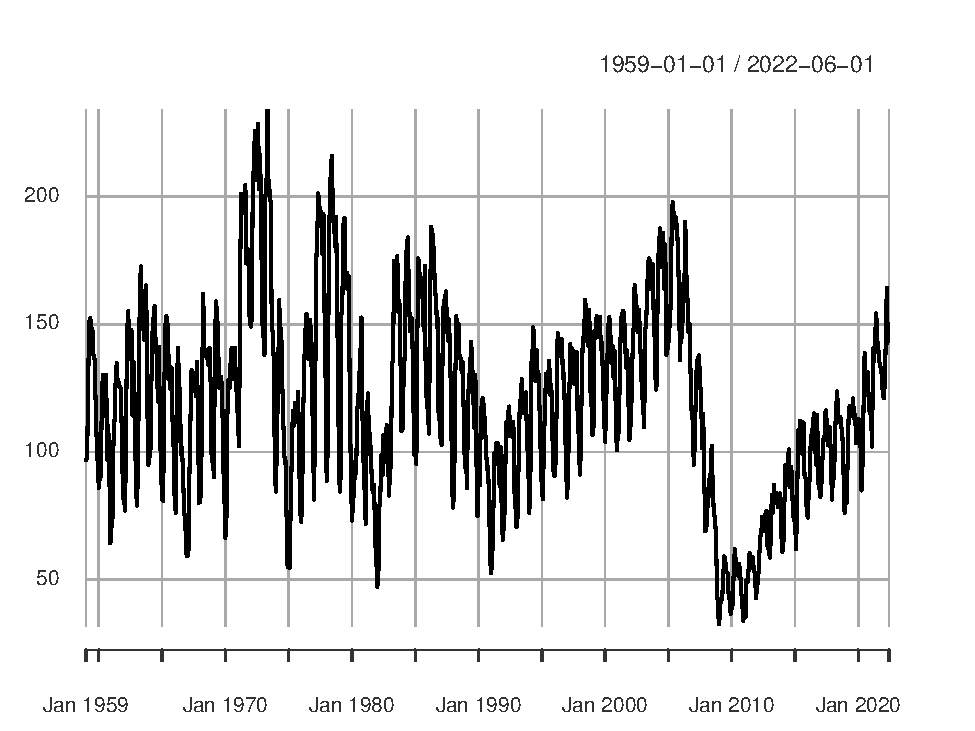
\includegraphics[width=0.8\linewidth]{bookdown-demo_files/figure-latex/ch5-figure4-1} 

}

\caption{Housing Starts in U.S.}\label{fig:ch5-figure4}
\end{figure}

One option to deal with seasonality is to either obtain seasonally adjusted data from the source itself. Alternatively, we can use decomposition method and appropriately filter out the seasonal component. However, if our objective is to explicitly model the seasonal component of a time series then we must work with non-seasonally adjusted data.

\hypertarget{regression-model-with-seasonal-dummy-variables}{%
\subsection{Regression Model with Seasonal Dummy Variables}\label{regression-model-with-seasonal-dummy-variables}}

One way to account for seasonal patterns in data is to add dummy variables for season. To avoid perfect multicollinearity, is there are \(s\) seasons, we can include \(s-1\) dummy variables. For example, for quarterly data, \(s=4\) and hence we need \(s-1=3\) dummy variables in our regression model. Formally, for quarterly data, the seasonal regression model is given by:

\begin{equation}
y_t= \beta_0 + \beta_1 D_{1t}+ \beta_2 D_{2t} + \beta_3 D_{3t} + \epsilon_t
\end{equation}

In the above regression model, \(D_1,D_2,\) and \(D_3\) are dummy variables that capture first three quarters of the year. For example, \(D_1=1\) for the first quarter and \(D_1=0\) otherwise. Similarly, \(D_2=1\) for the second quarter and \(D_2=0\) otherwise. In this example, we use the fourth quarter as the \emph{base group}.

The above model can be estimated using OLS. Again, we can use the residual from our estimated model as a measure of \emph{deseasonlized} data. We can also forecast the dependent variable based on the seasonal component only.

\hypertarget{application-seasonal-model-of-housing-starts}{%
\subsection{Application: Seasonal Model of Housing Starts}\label{application-seasonal-model-of-housing-starts}}

We now estimate a seasonal regression model for the housing starts data presented in Figure \ref{fig:ch5-figure4}. The data is at monthly frequency which implies we can have 12 possible seasons and hence would need 11 dummy variables in our regression model. Formally, we use January as the base group and include dummy variables for the last 11 months of the year:

\begin{equation}
y_t=\beta_0 + \sum_{i=2}^{12}\beta_i D_{it} + \epsilon_t
\end{equation}

Table \ref{tab:ch5-table3} presents the estimation results for this exercise. In Figure \ref{fig:ch5-figure5} we plot the forecast of housing starts for next 12 months using our estimated model, along with 95\% confidence bands.

\begin{table}[t]

\caption{\label{tab:ch5-table3}Regression Results}
\centering
\begin{tabular}{lcccc}
\toprule
  & Estimate & Std. Error & t value & Pr(>|t|)\\
\midrule
(Intercept) & 86.925 & 4.328 & 20.082 & 0.000\\
season2 & 2.941 & 6.121 & 0.480 & 0.631\\
season3 & 31.936 & 6.121 & 5.217 & 0.000\\
season4 & 48.499 & 6.147 & 7.890 & 0.000\\
season5 & 53.734 & 6.147 & 8.742 & 0.000\\
\addlinespace
season6 & 52.697 & 6.147 & 8.573 & 0.000\\
season7 & 46.960 & 6.147 & 7.640 & 0.000\\
season8 & 44.849 & 6.147 & 7.296 & 0.000\\
season9 & 38.210 & 6.147 & 6.216 & 0.000\\
season10 & 42.242 & 6.147 & 6.872 & 0.000\\
\addlinespace
season11 & 21.104 & 6.147 & 3.433 & 0.001\\
season12 & 4.797 & 6.147 & 0.780 & 0.435\\
\bottomrule
\end{tabular}
\end{table}

\begin{verbatim}
## Error in forecast(fit, h = 12): unused argument (h = 12)
\end{verbatim}

\begin{verbatim}
## Error in plot(fcast, include = 24, main = ""): object 'fcast' not found
\end{verbatim}

\hypertarget{modeling-cycle}{%
\chapter{Modeling Cycle}\label{modeling-cycle}}

In this chapter we will focus on the cyclical component of a time series and hence focus on data that either has no trend and seasonal components, or data that is filtered to eliminate any trend and seasonality. One of the most commonly used method to model cyclicality is the \emph{Autogressive Moving Average (ARMA)}. This model has two distinct components:

\begin{enumerate}
\def\labelenumi{\arabic{enumi}.}
\item
  \emph{Autoregressive (AR) component}: the current period value of a time series variable depends on its past (lagged) observations. We use \(p\) to denote the \textbf{order} of the AR component and is the number of lags of a variable that directly affect the current period value. For example, a firm's production in the current period maybe impacted by past levels of production. If last year's production exceeded demand, the stock of unsold goods may be used to meet this period demand first, hence lowering the current period production.
\item
  \emph{Moving average (MA) component}: the current period value of a time series variable depends on current period \textbf{shock} as well as past shocks to this variable. We use \(q\) to denote the \textbf{order} of the MA component and is the number of past period shocks that affect the current period value of the variable of interest. For example, if the Federal Reserve Bank raises the interest in 2016, the effects of that policy shock may impact investment and consumption spending in 2017.
\end{enumerate}

Before we consider these time series model in details it is useful to discuss certain properties of time series that allow us a better understanding of these models.

\hypertarget{stationarity-and-autocorrelation}{%
\section{Stationarity and Autocorrelation}\label{stationarity-and-autocorrelation}}

\hypertarget{covariance-stationary-time-series}{%
\subsection{Covariance Stationary Time Series}\label{covariance-stationary-time-series}}

\BeginKnitrBlock{definition}[Covariance Stationary Time Series]
\protect\hypertarget{def:d7}{}{\label{def:d7} \iffalse (Covariance Stationary Time Series) \fi{} }
\EndKnitrBlock{definition}

A time series \(\{y_t\}\) is said to be a \emph{covariance stationary process} if:

\begin{enumerate}
\def\labelenumi{\arabic{enumi}.}
\tightlist
\item
  \(E(y_t)=\mu_y \quad \forall \quad t\)
\item
  \(Var(y_t)=\sigma_y^2 \quad \forall \quad t\)
\item
  \(Cov(y_t,y_{t-s})=\gamma(s) \quad \forall \quad s\neq t\)
\end{enumerate}

One way to think about stationarity is \emph{mean-reversion}, i.e, the tendency of a time series to return to its \emph{long-run} unconditional mean following a shock (or a series of shock). Figure @\ref(fig:ch6-figure1) below shows this property graphically.

\begin{figure}

{\centering 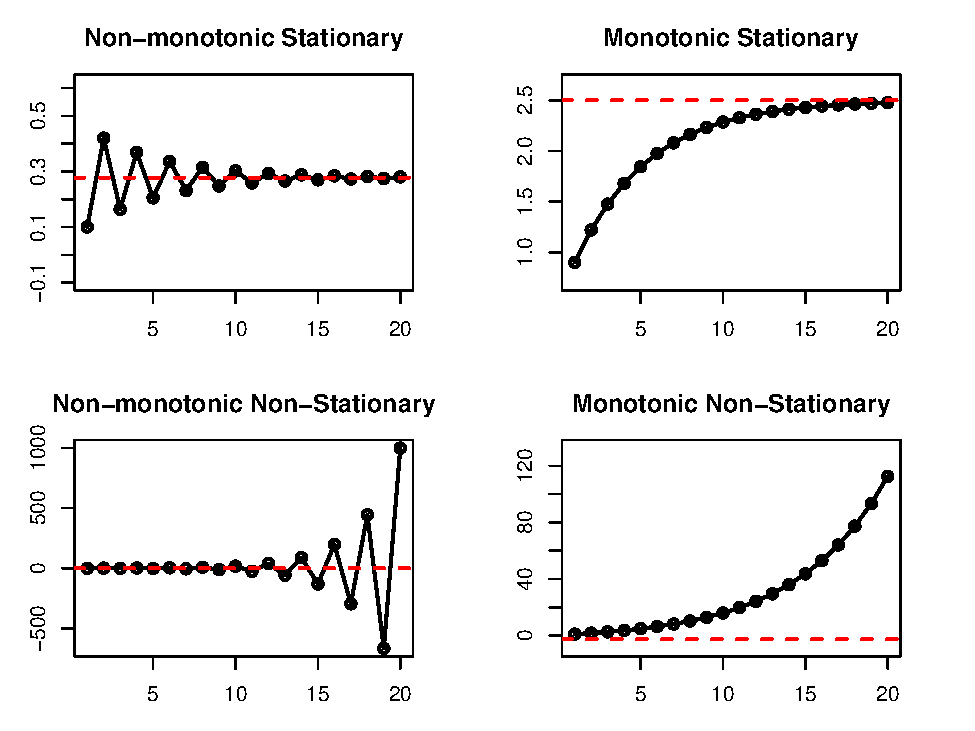
\includegraphics[width=0.8\linewidth]{bookdown-demo_files/figure-latex/ch6-figure1-1} 

}

\caption{Reversion to mean}\label{fig:ch6-figure1}
\end{figure}

\begin{figure}

{\centering 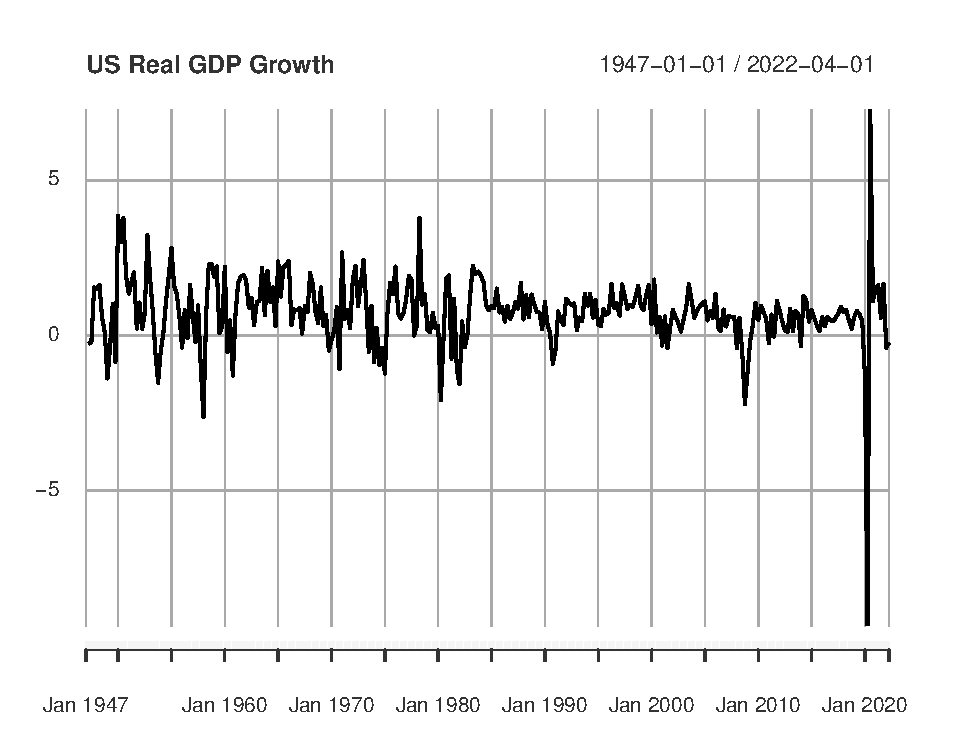
\includegraphics[width=0.8\linewidth]{bookdown-demo_files/figure-latex/ch6-figure2-1} 

}

\caption{Reversion to mean in practice}\label{fig:ch6-figure2}
\end{figure}

In practice however, you will not be able to visualize a mean-reverting stationary process this clearly. For example, in Figure \ref{fig:ch6-figure2} we plot real GDP growth for the U.S. which is a stationary process with a mean of 0.7\%. In this chapter we will only consider stationary time series data. Later on we will learn how to work with non-stationary data.

\hypertarget{correlation-vs-autocorrelation}{%
\subsection{Correlation vs Autocorrelation}\label{correlation-vs-autocorrelation}}

In statistics, correlation is a measure of relationship between two variables. In the time series setting, we can think of the current period value and the past period value of a variable as two \textbf{separate} variables, and compute correlation between them. Such a correlation, between current and lagged observation of a time series is called \textbf{serial correlation} or \textbf{autocorrelation}. In general, for a time series, \(\{y_t\}\), the autocorrelation is given by:

\begin{align}
    Cor(y_t,y_{t-s})=\frac{ Cov(y_t,y_{t-s})}{\sqrt{\sigma^2_{y_t} \times \sigma^2_{y_{t-s}}}}
        \end{align}
where \(Cov(y_t,y_{t-s})= E(y_t-\mu_{y_t})(y_{t-s}-\mu_{y_{t-s}})\) and \(\sigma^2_{y_t}=E(y_t-\mu_{y_t})^2\)

For a stationary time series, using the three conditions the \textbf{Autocorrelation Function (ACF)} denoted by \(\rho(s)\) is given by:

\begin{align}
    ACF(s) \ or \ \rho(s)=\frac{\gamma(s)}{\gamma(0)}
    \end{align}

Non-zero values of the ACF indicates presences of serial correlation in the data. Figure \ref{fig:ch6-figure3} shows the ACF for a stationary time series with positive serial correlation. If your data is stationary then the ACF should eventually converge to 0. For a non-stationary data, the ACF function will not decay over time.

\begin{figure}

{\centering 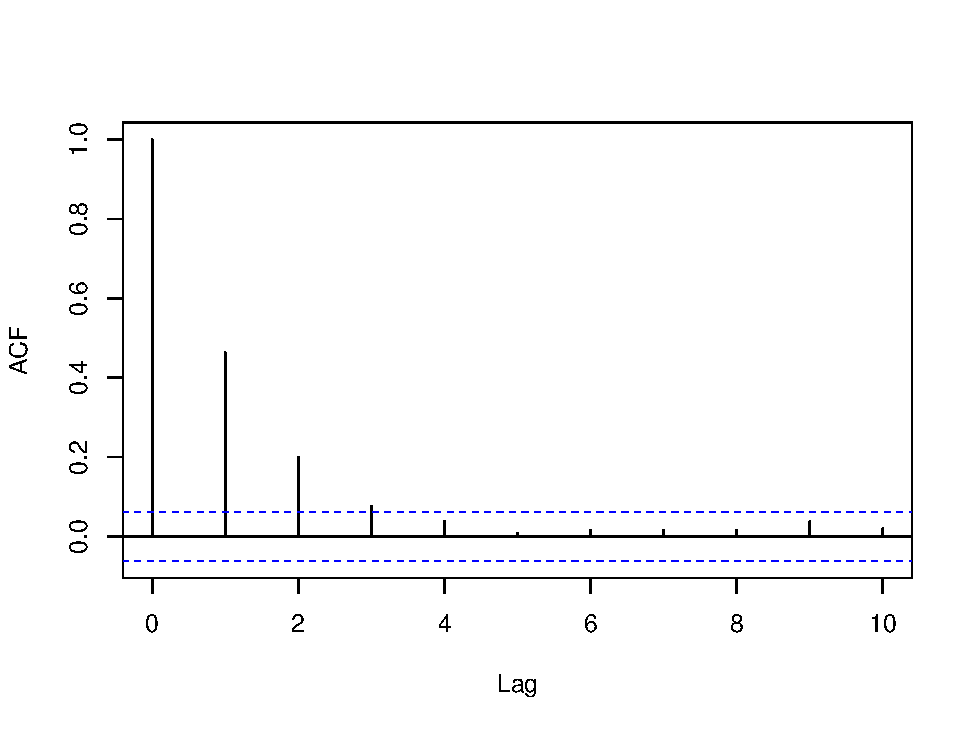
\includegraphics[width=0.8\linewidth]{bookdown-demo_files/figure-latex/ch6-figure3-1} 

}

\caption{ACF for a Stationary Time Series}\label{fig:ch6-figure3}
\end{figure}

\hypertarget{partial-autocorrelation}{%
\subsection{Partial Autocorrelation}\label{partial-autocorrelation}}

\BeginKnitrBlock{definition}[Partial Auto Correlation Function (PACF)]
\protect\hypertarget{def:d9}{}{\label{def:d9} \iffalse (Partial Auto Correlation Function (PACF)) \fi{} }
\EndKnitrBlock{definition}

The ACF captures the relationship between the current period value of a time series and all of its past observations. It includes both direct as well as indirect effects of the past observations on the current period value. Often times it is of interest to measure the direct relationship between the current and past observations, \textbf{partialing} out all indirect effects. The \emph{partial autocorrelation function (PACF)} for a stationary time series \(y_t\) at lag \(s\) is the direct correlation between \(y_t\) and \(y_{t-s}\), after filtering out the linear influence of \(y_{t-1},\ldots,y_{t-s-1}\) on \(y_t\). Figure \ref{fig:ch6-figure4} below shows the PACF for a stationary time series where only one lag directly affects the time series in the current period.

\begin{figure}

{\centering 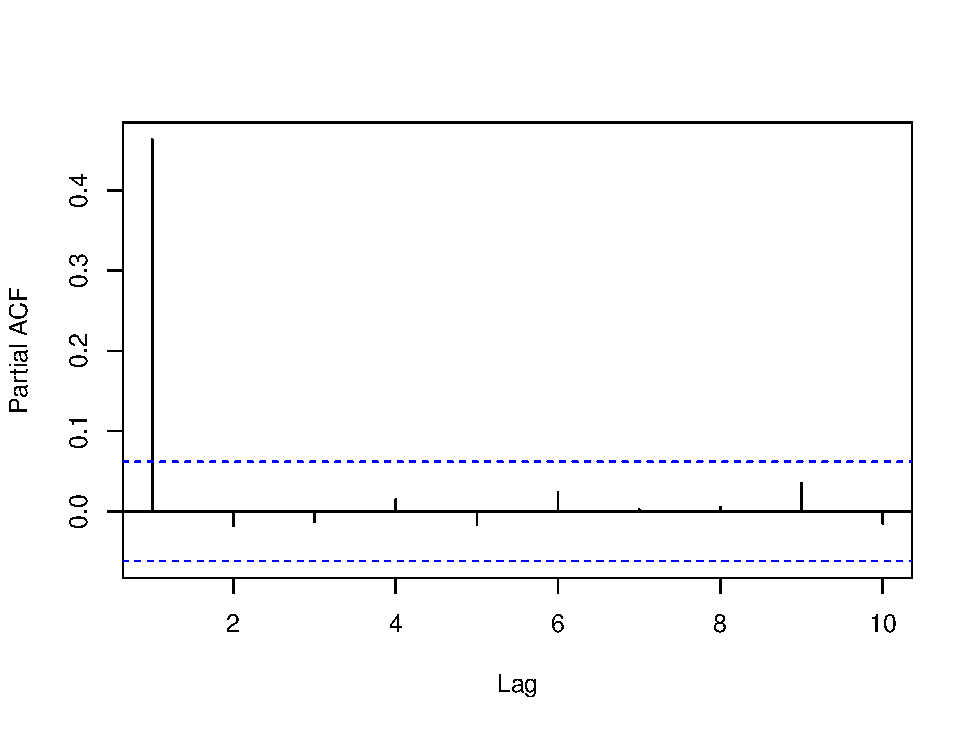
\includegraphics[width=0.8\linewidth]{bookdown-demo_files/figure-latex/ch6-figure4-1} 

}

\caption{PACF for a Stationary Time Series}\label{fig:ch6-figure4}
\end{figure}

\hypertarget{lag-operator}{%
\subsection{Lag operator}\label{lag-operator}}

A \textbf{lag operator} denoted by \(L\) allows us to write ARMA models in a more concise way. Applying lag operator once moves the time index by one period; applying it twice moves the time index back by two period; applying it \(s\) times moves the index back by \(s\) periods.
\[ Ly_t=y_{t-1} \]
\[ L^2y_t=y_{t-2} \]
\[ L^3y_t=y_{t-3} \]
\[\vdots\]
\[ L^sy_t=y_{t-s} \]

\hypertarget{autoregressive-ar-model}{%
\section{Autoregressive (AR) Model}\label{autoregressive-ar-model}}

A \emph{stationary}time series \(\{x_t\}\) can be modeled as an AR process. In general, an AR(p) model is given by:

\begin{equation}
 y_t = \phi_0 +\phi_1 y_{t-1} + \phi_2 y_{t-2} + ...... + \phi_p y_{t-p}+\epsilon_t
 \end{equation}

Here \(\phi_i\) captures the effect of \(y_{t-i}\) on \(y_t\). The order of the AR process is not known apriori. It is common to use either AIC or BIC to determine the optimal lag length for an AR process.

Using the Lag operator, we can rewrite the above AR(p) model as follows:
\[ \Phi(L)y_t=\phi_0+\epsilon_t \]

where \(\displaystyle \Phi(L)\) is a polynomial of degree \(p\) in L:

\[ \Phi(L) = 1-\phi_1 L - \phi_2 L^2- \ldots\ldots\ldots\ldots -\phi_p L^p\]

For example, an AR(1) model can be written as:
\[y_t=\phi_0+\phi_1 y_{t-1} + \epsilon_t \Rightarrow  \Phi(L)y_t=\phi_0+\epsilon_t\]
where,
\[ \Phi(L) = 1-\phi_1 L \]

\textbf{Characteristic equation}: A characteristic equation is given by:

\[\Phi(L)=0\]

The roots of this equation play an important role in determining the dynamic behavior of a time series.

\hypertarget{unit-root-and-stationarity}{%
\subsection{Unit root and Stationarity}\label{unit-root-and-stationarity}}

For a time series to be stationary there should be no \textbf{unit root} in its \emph{characteristic equation}. In other words, all roots of the characteristic equation must fall outside the unit circle. Consider the following AR(1) model:
\[\Phi(L)y_t = \phi_0 + \epsilon_t\]

The characteristic equation is given by:
\[\Phi(L)=1-\phi_1L=0 \]

The root that satisfies the above equation is:
\[ L^*=\frac{1}{\phi_1}\]

For no unit root to be present, \(L^*>|1|\) which implies that \(|\phi_1|<1\).

Typically, for any AR process to be stationary, some restrictions will be imposed on the values of \(\phi_i's\), the coefficients of the lagged variables in the model.

\hypertarget{properties-of-an-ar1-model}{%
\subsection{Properties of an AR(1) model}\label{properties-of-an-ar1-model}}

A stationary AR(1) model is given by:
\[ y_t=\phi_0 +\phi_1 y_{t-1}+ \epsilon_t \quad ; \ \epsilon_t\sim WN(0, \sigma_\epsilon^2) \ and \  |\phi_1|<1\]

\begin{enumerate}
\def\labelenumi{\arabic{enumi}.}
\item
  \(\displaystyle \phi_1\) measures the persistence in data. A larger value indicates shocks to \(y_t\) dissipate slowly over time.
\item
  Stationarity of \(y_t\) implies certain restrictions on the AR(1) model.

  \begin{enumerate}
  \def\labelenumii{\roman{enumii}.}
  \tightlist
  \item
    Constant long run mean: is the unconditional expectation of \(y_t\):
    \[ E(y_t) = \mu_y= \frac{\phi_0}{1-\phi_1}  \]
  \item
    Constant long run variance: is the unconditional variance of \(y_t\):
    \[ Var(y_t)=\sigma^2_y= \frac{\sigma^2_\epsilon}{1-\phi_1^2}\]
  \item
    ACF function:
    \[ \rho(s) = \phi_1^s\]
  \item
    PACF function:
    \begin{equation*}
      PACF(s) =
      \begin{cases}
    \phi_1 & \text{if  s=1}\\
    0 & \text{if s>1}
      \end{cases}
     \end{equation*}
  \end{enumerate}
\end{enumerate}

\hypertarget{estimating-an-ar-model}{%
\section{Estimating an AR model}\label{estimating-an-ar-model}}

When estimating the AR model we have two alternatives:

\begin{enumerate}
\def\labelenumi{\arabic{enumi}.}
\item
  OLS: biased (but consistent) estimates. Also, later on when we add MA components we cannot use OLS.
\item
  Maximum Likelihood Estimation (MLE): can be used to estimate AR as well as MA components
\end{enumerate}

\hypertarget{maximum-likelihood-estimation-mle}{%
\subsection{Maximum Likelihood Estimation (MLE)}\label{maximum-likelihood-estimation-mle}}

\begin{itemize}
\tightlist
\item
  MLE approach is based on the following idea:
\end{itemize}

\emph{what set of values of our parameters maximize the likelihood of observing our data if the model we have was used to generate this data.}

\textbf{Likelihood function}: is a function that gives us the probability of observing our data given a model with some parameters.

\hypertarget{likelihood-vs-probability}{%
\subsubsection{Likelihood vs Probability}\label{likelihood-vs-probability}}

Consider a simple example of tossing a coin. Let \(X\) denotes the random variable that is the outcome of this experiment being either heads or tails. Let \(\theta\) denote the probability of heads which implies \(1-\theta\) is the probability of obtaining tails. Here, \(\theta\) is our parameter of interest. Suppose we toss the coin 10 times and obtain the following data on \(X\):
\[X=\{H,H,H,H,H,H,T,T,T,T\}\]

Then, the probability of obtaining this sequence of X is given by:
\[Prob (X|\theta)=\theta^6 (1-\theta)^4\]

This is the probability distribution function the variable \(X\). As we change \(X\), we get a different probability for a given value of \(\theta\).

Now let us ask a different question. Once we have observed the sequence of heads and tails, lets call it our data which is fixed. Then, what is probability of observing this data, if our probability distribution function is given by the equation above? That gives us the likelihood function:

\[ L(\theta)=Prob(X|\theta)=\theta^6(1-\theta)^4\]

Note that with fixed \(X\), as we change \(\theta\) the likelihood of observing this data will change.

\textbf{This is an important point that distinguishes likelihood function from the probability distribution function. Although both have the same equation, the probability function is a function of the data with the value of the parameter fixed, while the likelihood function is a function of the parameter with the data fixed.}

\hypertarget{maximum-likelhood-estimation}{%
\subsubsection{Maximum Likelhood Estimation}\label{maximum-likelhood-estimation}}

Now we are in a position to formally define the likelihood function.

\BeginKnitrBlock{definition}
\protect\hypertarget{def:unnamed-chunk-4}{}{\label{def:unnamed-chunk-4} }Let \(X\) denotes a random variable with a given probability distribution function denoted by \(f(x_i|\theta)\). Let \(D=\{x_1, x_2,\dots,x_n\}\) denote a sample realization of \(X\). Then, the likelhood function, denoted by \(L(\theta)\) is given by:
\[L(\theta)=f(x_1,x_2,\dots,x_n|\theta)\]
\EndKnitrBlock{definition}

If we further assume that each realization of \(X\) is independent of the others, we get:
\[L(\theta)=f(x_1,x_2,\dots,x_n|\theta)=f(x_1|\theta)\times f(x_2|\theta) \times \dots \times f(x_n|\theta)\]

A mathematical simplification is to work with natural logs of the likelihood function, which assuming independently distributed random sample, gives us:

\[ lnL(\theta)=ln(f(x_1|\theta)\times f(x_2|\theta) \times \dots \times f(x_n|\theta))=\sum_{i=1}^{N}ln(f(x_i|\theta))\]

\BeginKnitrBlock{definition}
\protect\hypertarget{def:unnamed-chunk-5}{}{\label{def:unnamed-chunk-5} }The maximum likelihood estimator, denoted by \(\hat{\theta}_{MLE}\), maximizes the log likelihood function:
\[ \hat{\theta}_{MLE} \equiv arg \max_{\theta} lnL(\theta) \]
\EndKnitrBlock{definition}

\BeginKnitrBlock{example}
\protect\hypertarget{exm:unnamed-chunk-6}{}{\label{exm:unnamed-chunk-6} }Compute maximum likelihood estimator of \(\mu\) of an indpendently distributed random variable that is normally distributed with a mean of \(\mu\) and a variance of \(1\):

\[ f(y_t|\mu)=\frac{1}{\sqrt{2\pi}}e^{-\frac{1}{2} (y_t-\mu)^2}\]

Solution: The log likelihood function is given by:

\[lnL= -Tln2\pi-\frac{1}{2}\sum_{t=1}^T(y_t-\mu)^2 \]

From the first order condition, we get
\[ \frac{\partial LnL}{\partial \mu}=\sum_{t=1}^T(y_t-\mu)=0\Rightarrow \hat{\mu}_{MLE}=\frac{\sum_{t=1}^T y_t}{T}\]
\EndKnitrBlock{example}

\hypertarget{mle-of-an-arp-model}{%
\subsection{MLE of an AR(p) model}\label{mle-of-an-arp-model}}

One complication we face in estimating an AR(p) model is that by definition the realizations of the variable are not independent of each other. As a result we cannot simplify the likelihood function by multiplying individual probability density functions to obtain the joint probability density function, i.e.,
\[ f(y_1,y_2,\dots,y_T|\theta) \neq f(y_1|\theta)\times f(y_2|\theta)\times \dots \times f(y_T|\theta)\]

Furthermore, as the order of AR increases, the joint density function we need to estimate becomes even more complicated. In this class we will focus on the method that divides the joint density into the product of conditional densities and density of a set of initial values. The idea comes from the conditional probability formula for two related events \(A\) and \(B\):

\[ P(A|B) =\frac{P(\text{A and B})}{P(B)} \Rightarrow P(\text{A and B}) = P(A|B)\times P(B) \]

In the time series context, I will explain this for a stationary AR(1) model. We know that in this model only last period observation directly affects the current period value. Hence, consider the first two observations of a stationary time series: \(y_1\) and \(y_2\). Then the joint density of these adjacent observations is given by,

\[ f(y_1,y_2;\theta)= f(y_2|y_1; \theta)\times f(y_1;\theta)\]

Similarly, for the first three observations we get:

\[ f(y_1,y_2,y_3;\theta)= f(y_3|y_2; \theta)\times f(y_2|y_1; \theta) \times f(y_1; \theta)\]

Hence, for \(T\) observations we get:

\[ f(y_1,y_2,y_3, ...,y_T; \theta)= f(y_T|y_{T-1};\theta)\times f(y_{T-1}|y_{T-2}; \theta)\times.... \times f(y_1; \theta)\]

The log-likelihood function is given by:

\[ ln \ L(\theta) = ln \ f(y_1;\theta) + \sum_{t=2}^{T} ln \ f(y_t|y_{t-1}; \theta)  \]

We can then maximize the above likelihood function to obtain an MLE estimator for the AR(1) model.

\hypertarget{selection-of-optimal-order-of-the-ar-model}{%
\subsection{Selection of optimal order of the AR model}\label{selection-of-optimal-order-of-the-ar-model}}

Note that apriori we do not know the order of the AR model for any given time series. We can determine the optimal lag order by using either AIC or BIC. The process is as follows:

\begin{enumerate}
\def\labelenumi{\arabic{enumi}.}
\item
  Set \(p=p_{max}\) where \(p_{max}\) is an integer. A rule of thumb is to set
  \[p_{max}=integer\left[12\times \left(\frac{T}{100}\right)^{0.25}\right]\]
\item
  Estimate all AR models from \(p=1\) to \(p=p_{max}\).
\item
  Select the final model as the one with lowest AIC or lowest BIC.
\end{enumerate}

\hypertarget{forecasting-using-arp-model}{%
\subsection{Forecasting using AR(p) model}\label{forecasting-using-arp-model}}

Having estimated our AR(p) model with the optimal lag length, we can use the conditional mean to compute the forecast and conditional variance to compute the forecast errors. Consider an AR(1) model:

\[y_t=\phi_0+\phi_1 y_{t-1} +\epsilon_t\]

Then, the 1-period ahead forecast is given by:
\[f_{t,1}=E(y_{t+1}|\Omega_t)=\phi_0+\phi_1 y_t\]
Similarly, the 2-period ahead forecast is given by:
\[f_{t,2}=E(y_{t+2}|\Omega_t)=\phi_0+\phi_1 E(y_{t+1}|\Omega_t) =\phi_0+\phi_1f_{t,1}\]

In general, we can get the following recursive forecast equation for h-period's ahead:
\[f_{t,h}=\phi_0+\phi_1 f_{t,h-1}\]

Correspondingly, the h-period ahead forecast error is given by:
\[e_{t,h}=y_{t+h}- f_{t,h}=\epsilon_{t+h}+\phi_1 e_{t,h-1}\]

\BeginKnitrBlock{theorem}
\protect\hypertarget{thm:unnamed-chunk-7}{}{\label{thm:unnamed-chunk-7} }The h-period ahead forecast converges to the unconditional mean of \(y_t\), i.e., \[\lim_{h\to\infty} f_{t,h}=\mu_y=\frac{\phi_0}{1-\phi_1}\]
\EndKnitrBlock{theorem}

\BeginKnitrBlock{theorem}
\protect\hypertarget{thm:unnamed-chunk-8}{}{\label{thm:unnamed-chunk-8} }The variance of the h-period ahead forecast error converges to the unconditional variance of \(y_t\), i.e., \[\lim_{h\to\infty} Var(e_{t,h})=\sigma^2_y=\frac{\sigma^2_\epsilon}{1-\phi_1^2}\]
\EndKnitrBlock{theorem}

\hypertarget{moving-average-ma-model}{%
\section{Moving Average (MA) Model}\label{moving-average-ma-model}}

Another commonly used method for capturing the cyclical component of the time series is the \textbf{moving average (MA)} model where the current value of a time series linearly depends on current and past shocks. Formally, a \emph{stationary} time series \(\{y_t\}\) can be modeled as an MA(q) process:
\begin{equation}
  y_t = \theta_0 + \epsilon_t + \theta_1 \epsilon_{t-1} + \theta_2 \epsilon_{t-2} + ...... + \theta_q \epsilon_{t-q}
    \end{equation}

Using lag operator, we can write this in more compact form as:

\[y_t = \theta_0 +\Theta(L) \epsilon_t\]

where \(\Theta(L)=1+\theta_1 L+ \theta_2 L^2+...+\theta_q L^q\) is lag polynomial of order \(q\).

Note that because each one of the current and past shocks are white noise processes, an MA(q) model is always stationary.

\hypertarget{invertibility-of-an-ma-process}{%
\subsection{Invertibility of an MA process}\label{invertibility-of-an-ma-process}}

Consider the following MA(1) process with\(\theta_0=0\) for simplicity:
\[y_t=\epsilon_t +\theta_1 \epsilon_{t-1}\]

Using the lag operator we can rewrite this equation as follows:

\[y_t= (1+\theta_1L)\epsilon_t \Rightarrow y_t(1+\theta_1 L) ^{-1}=\epsilon_t\]

Note that if \(|\theta_1|<1\), then we can use the Taylor series expansion centered at 0 and get:

\[(1+\theta_1 L)^{-1}=1-\theta_1 L+(\theta_1L)^2-(\theta_1L)^3+ (\theta_1L)^4-...... \]

Hence, an MA(1) can be rewritten as follows:

\[y_t (1-\theta_1 L+(\theta_1L)^2-(\theta_1L)^3+ (\theta_1L)^4-......)=\epsilon_t\]
\[\Rightarrow y_t -\theta_1 y_{t-1} +\theta_1^2y_{t-2}-\theta_1^3 y_{t-3}....=\epsilon_t\]

Rearranging terms, we get the \(AR(\infty)\) representation for an invertible MA(1) model:
\[y_t=-\sum_{i=1}^{\infty}(-\theta_1)^i \ y_{t-i}+\epsilon_t\]

\BeginKnitrBlock{definition}
\protect\hypertarget{def:unnamed-chunk-9}{}{\label{def:unnamed-chunk-9} }An MA process is invertible if it can be represented as a stationary \(AR(\infty)\).
\EndKnitrBlock{definition}

\hypertarget{properties-of-an-invetible-ma1}{%
\subsection{Properties of an invetible MA(1)}\label{properties-of-an-invetible-ma1}}

An invertible MA(1) model is given by:

\[ y_t = \theta_0 + \epsilon_t + \theta_1 \epsilon_{t-1} \quad ; \ \epsilon_t\sim WN(0, \sigma_\epsilon^2) \ and \  |\theta_1|<1\]

\begin{enumerate}
\def\labelenumi{\arabic{enumi}.}
\item
  Constant unconditional mean of \(y_t\):
  \[E(y_t)=\mu_y =\theta_0 \]
\item
  Constant unconditional variance of \(y_t\):
\end{enumerate}

\[Var(y_t)=\sigma^2_y=\sigma^2_\epsilon(1+\theta_1^2)\]

\begin{enumerate}
\def\labelenumi{\arabic{enumi}.}
\setcounter{enumi}{2}
\item
  ACF function:
  \begin{equation*}
    ACF(s) =
    \begin{cases}
   \frac{\theta_1}{1+\theta_1^2} & \text{if  s=1}\\
   0 & \text{if s>1}
    \end{cases}
   \end{equation*}
\item
  PACF function: using the invertibility it is evident that PACF of an MA(1) decays with \(s\).
\end{enumerate}

\hypertarget{forecast-based-on-maq}{%
\subsection{Forecast based on MA(q)}\label{forecast-based-on-maq}}

Like before, the h-period ahead forecast is the conditional expected value of the time series. Consider an MA(1) model:

\[y_t=\theta_0 +\epsilon_t + \theta_1 \epsilon_{t-1}\]

Then, the 1-period ahead forecast is given by:

The h-period ahead forecast for \(h>1\) is given by:
\[f_{t,h}=E(y_{t+h}|\Omega_t)=\theta_0\]

In general, for an MA(q) model, the forecast for \(h>q\) is the long run mean \(\theta_0\). This is why we say that an MA(q) process has a memory of \emph{q} periods.

\hypertarget{armap-q}{%
\section{ARMA(p, q)}\label{armap-q}}

An ARMA model simply combines both AR and MA components to model the dynamics of a time series. Formula,

\begin{equation}
   y_t = \phi_0 +\phi_1 y_{t-1} + \phi_2 y_{t-2} + ...... + \phi_p y_{t-p}+\epsilon_t + \theta_1 \epsilon_{t-1} + \theta_2 \epsilon_{t-2} + ...... + \theta_q \epsilon_{t-q}
   \end{equation}

Note that:

\begin{enumerate}
\def\labelenumi{\arabic{enumi}.}
\item
  Estimation is done by maximum likelihood method.
\item
  Optimal order for AR and MA components is selected using AIC and/or BIC.
\item
  The forecast of \(y_t\) from an ARMA(p,q) model will be dominated by the AR component for \(h>q\). To see this consider the following ARMA(1,1) model:
\end{enumerate}

\[y_t = \phi_0 +\phi_1 y_{t-1}+ \epsilon_t + \theta_1 \epsilon_{t-1}\]

Then, the 1-period ahead forecast is:
\[f_{t,1} = E(y_{t+1}|\Omega_t) = \phi_0 + \phi_1 y_t + \theta_1 \epsilon_{t-1}\]

Here both MA and AR component affect the forecast. But now consider the 2-period ahead forecast:

\[f_{t,2} = E(y_{t+2}|\Omega_t) = \phi_0 + \phi_1 f_{t,1}\]

Hence, no role is played by the MA component in determining the 2-period ahead forecast. For any \(h>1\) only the AR component affects the forecast from this model.

\hypertarget{integrated-arma-or-arimapdq}{%
\section{Integrated ARMA or ARIMA(p,d,q)}\label{integrated-arma-or-arimapdq}}

Thus far we have assumed that our data is stationary. However, often we may find that this assumption is not supported in practice. In such a case we need to tranform our data appropriately before estimating an ARMA model. The procedure can be summarized as follows:

\begin{enumerate}
\def\labelenumi{\arabic{enumi}.}
\item
  Determine whether there is a unit root in data or not. Presence of unit root indicates non-stationarity. We will use Augmented Dickey-Fuller (ADF) test for this purpose.
\item
  If data is non-stationary, then we need to appropriately transform our data to make it stationary.
\item
  Once we have obtained a stationary transformation of our original data, we can proceed and estimate the ARMA model as before.
\end{enumerate}

\hypertarget{trend-stationary-vs-difference-stationary-time-series}{%
\section{Trend Stationary vs Difference Stationary Time Series}\label{trend-stationary-vs-difference-stationary-time-series}}

There are two types of time series we often encounter in real world:

\begin{enumerate}
\def\labelenumi{\arabic{enumi}.}
\tightlist
\item
  Trend-stationary: a time-series variable is non-stationary becuase it has a deterministic trend. Once we detrend our data then it will become stationary. In this case the appropriate transformation is to estimate a trend model and then use the residual as the detrended stationary data. For example, suppose our data has a linear trend given by:
\end{enumerate}

\[y_t = \beta_0 +\beta_1 t +\epsilon_t\]

Then the OLS residual from this model, \(e_t=y_t-\hat{y_t}\) is the detrended \(y_t\) which will be stationary. Hence, we will estimate an ARMA(p,q) model using this detrended variable.

\begin{enumerate}
\def\labelenumi{\arabic{enumi}.}
\setcounter{enumi}{1}
\tightlist
\item
  Difference-stationary: a time-series variable is non-stationary because it contains a stochastic trend. Here, the transformation requires us to difference the orignial data until we obtain a stationary time series. Let \(d\) denote the minimum number of differences needed to obtain a stationary time series:
\end{enumerate}

\[\Delta_d \ y_t=(1-L)^d \ y_t\]

In this case, we say that \(y_t\) is intergrated of order \(d\) or more formally, \(y_t\) is an \(I(d)\) process. Hence, for \(d=1\) we obtain an \(I(1)\) process implying that:

\[\Delta_1 \ y_t=(1-L)^1 \ y_t=y_t-y_{t-1} \quad  \text{is stationary}\]

In otherwords, the first difference of an I(1) process is stationary. Similarly for \(d=2\), we obtain an \(I(2)\) process where second difference will be stationary and so forth.

\hypertarget{testing-for-a-unit-root}{%
\section{Testing for a unit root}\label{testing-for-a-unit-root}}

Consider the following AR(1) model with no trend and intercept:

\[y_t=\phi_1 y_{t-1} +\epsilon_t  \ quad ; \epsilon_t\sim WN(0,\sigma^2_\epsilon)\]

We know that if \(\phi_1=1\) we have a unit root in this data. Lets subtract \(y_{t-1}\) from both sides and rewrite this model as:

\[y_t-y_{t-1}= (\phi_1-1)y_{t-1}+\epsilon_t \]

Define \(\rho=phi_1-1\). Then, we get:
\[\Delta y_t= \rho \ y_{t-1}+\epsilon_t \]

We can now estimate the above model and carry out the following test known as the Dickey-Fuller (DF) test:

\[H_0: \rho=0 \]
\[H_A: \rho<0\]

If the null hypothesis is not rejected, then we do not have sample evidence against the statement that \(\rho=0 \Rightarrow \phi_1=1\). Hence, we conclude that there is no evidence against the statement that there is unit root in the data. In contrast, if we reject the null hypothesis, then we can conclude that there is no unit root and hence the data is stationary.

The t- statistic is for the above test is denoted by \(\tau_1\) and is given by:
\[\tau_1 =\frac{\hat{\rho}}{se(\hat{\rho})}\]

Under the null hypothesis this test statistic follows the DF-distribution and the critical values are provided in most statistical softwares. Given that this is a left-tail test, the decision rule is that if the test statistic is less than the critical value then we reject the null hypothesis.

There are two issues we face when implementing this test in practice:

\begin{enumerate}
\def\labelenumi{\arabic{enumi}.}
\item
  First, the above procedure assumes that there is no intercept and trend in the data. In real world, we cannot make that assumption and must extend the test procedure to accomodate a non-zero intercept and trend. Hence, we have the following two additional versions of the DF test:

  \begin{enumerate}
  \def\labelenumii{\roman{enumii}.}
  \tightlist
  \item
    Constant and no trend model: Here our AR(1) model is
  \end{enumerate}

  \[\Delta y_t= \phi_0 + \rho \ y_{t-1}+\epsilon_t \]

  Now we can do two possible tests. The first test is that of the unit root:

  \[H_0: \rho=0 \]
  \[H_A: \rho<0\]

  The t statistic for this test is denoted by \(\tau_2\) and is given by:
  \[\tau_2 =\frac{\hat{\rho}}{se(\hat{\rho})}\]

  If the test statisitic is less than the critical value, we reject the null.

  The second test we can do is:
  \[H_0: \rho=\phi_0=0 \]
  \[H_A: Not \ H_0\]
  The test statistic for this test is denoted by \(\phi_1\). If the test statistic exceeds the critical value then we reject the null.

  \begin{enumerate}
  \def\labelenumii{\roman{enumii}.}
  \setcounter{enumii}{1}
  \tightlist
  \item
    Constant and linear trend model: Here our AR(1) model is
  \end{enumerate}

  \[\Delta y_t= \phi_0 + \beta \ t+ \rho \ y_{t-1}+\epsilon_t \]

  Now we can do three possible tests. The first test is that of the unit root;
  \[H_0: \rho=0 \]
  \[H_A: \rho<0\]
  The t statistic for this test is denoted by \(\tau_3\) and is given by:

  \[\tau_3 =\frac{\hat{\rho}}{se(\hat{\rho})}\]

  If the test statisitic is less than the critical value, we reject the null.

  The second test is:
  \[H_0: \rho=\phi_0=\beta=0 \]
  \[H_A: Not \ H_0\]
  The test statistic for this test is denoted by \(\phi_2\). If the test statistic exceeds the critical value then we reject the null.

  Finally the third test is:
  \[H_0: \rho=\beta=0 \]
  \[H_A: Not \ H_0\]
  The test statistic for this test is denoted by \(\phi_3\). If the test statistic exceeds the critical value then we reject the null.
\item
  Second, we only have allowed for AR(1). We need to extend the above testing procedure for higher order AR models. The Augmented DF (ADF) test allows for higher order lags in testing for a unit root. For example, the model with an intercept, trend, and \(p\) lags is given by:
  \[\Delta y_t= \phi_0 + \beta \ t+ \rho \ y_{t-1}+\sum_{i=2}^p\delta_i  y_{t-i}+\epsilon_t  \quad where \ \rho=\sum_{i=1}^p \phi_i-1\]
\end{enumerate}

\hypertarget{testing-for-unit-root-in-usdcad-exchange-rate}{%
\subsection{Testing for unit root in USD/CAD exchange rate}\label{testing-for-unit-root-in-usdcad-exchange-rate}}

In this application we will test for unit root in US-Canada exchange rate. For this purpose we work with monthly data from Jan 1971 through Oct 2018. Below I show the results for 3 models using the \textbf{urca} package in R.

\begin{verbatim}
## 
## ############################################### 
## # Augmented Dickey-Fuller Test Unit Root Test # 
## ############################################### 
## 
## Test regression none 
## 
## 
## Call:
## lm(formula = z.diff ~ z.lag.1 - 1 + z.diff.lag)
## 
## Residuals:
##       Min        1Q    Median        3Q       Max 
## -0.069547 -0.008871  0.000358  0.010441  0.124996 
## 
## Coefficients:
##             Estimate Std. Error t value Pr(>|t|)    
## z.lag.1    0.0001959  0.0005796   0.338    0.736    
## z.diff.lag 0.2758988  0.0400346   6.892 1.45e-11 ***
## ---
## Signif. codes:  0 '***' 0.001 '**' 0.01 '*' 0.05 '.' 0.1 ' ' 1
## 
## Residual standard error: 0.01717 on 577 degrees of freedom
## Multiple R-squared:  0.07658,    Adjusted R-squared:  0.07337 
## F-statistic: 23.92 on 2 and 577 DF,  p-value: 1.043e-10
## 
## 
## Value of test-statistic is: 0.3379 
## 
## Critical values for test statistics: 
##       1pct  5pct 10pct
## tau1 -2.58 -1.95 -1.62
\end{verbatim}

\begin{verbatim}
## 
## ############################################### 
## # Augmented Dickey-Fuller Test Unit Root Test # 
## ############################################### 
## 
## Test regression drift 
## 
## 
## Call:
## lm(formula = z.diff ~ z.lag.1 + 1 + z.diff.lag)
## 
## Residuals:
##       Min        1Q    Median        3Q       Max 
## -0.067687 -0.009468 -0.000592  0.010039  0.123436 
## 
## Coefficients:
##              Estimate Std. Error t value Pr(>|t|)    
## (Intercept)  0.010401   0.005319   1.955   0.0510 .  
## z.lag.1     -0.008173   0.004319  -1.892   0.0589 .  
## z.diff.lag   0.279076   0.039970   6.982 8.04e-12 ***
## ---
## Signif. codes:  0 '***' 0.001 '**' 0.01 '*' 0.05 '.' 0.1 ' ' 1
## 
## Residual standard error: 0.01713 on 576 degrees of freedom
## Multiple R-squared:  0.08169,    Adjusted R-squared:  0.0785 
## F-statistic: 25.62 on 2 and 576 DF,  p-value: 2.192e-11
## 
## 
## Value of test-statistic is: -1.8924 1.9691 
## 
## Critical values for test statistics: 
##       1pct  5pct 10pct
## tau2 -3.43 -2.86 -2.57
## phi1  6.43  4.59  3.78
\end{verbatim}

\begin{verbatim}
## 
## ############################################### 
## # Augmented Dickey-Fuller Test Unit Root Test # 
## ############################################### 
## 
## Test regression trend 
## 
## 
## Call:
## lm(formula = z.diff ~ z.lag.1 + 1 + tt + z.diff.lag)
## 
## Residuals:
##       Min        1Q    Median        3Q       Max 
## -0.067715 -0.009336 -0.000484  0.009933  0.123282 
## 
## Coefficients:
##               Estimate Std. Error t value Pr(>|t|)    
## (Intercept)  1.040e-02  5.324e-03   1.954   0.0512 .  
## z.lag.1     -8.356e-03  4.448e-03  -1.879   0.0608 .  
## tt           7.638e-07  4.386e-06   0.174   0.8618    
## z.diff.lag   2.793e-01  4.002e-02   6.978 8.25e-12 ***
## ---
## Signif. codes:  0 '***' 0.001 '**' 0.01 '*' 0.05 '.' 0.1 ' ' 1
## 
## Residual standard error: 0.01714 on 575 degrees of freedom
## Multiple R-squared:  0.08174,    Adjusted R-squared:  0.07695 
## F-statistic: 17.06 on 3 and 575 DF,  p-value: 1.257e-10
## 
## 
## Value of test-statistic is: -1.8787 1.3206 1.8027 
## 
## Critical values for test statistics: 
##       1pct  5pct 10pct
## tau3 -3.96 -3.41 -3.12
## phi2  6.09  4.68  4.03
## phi3  8.27  6.25  5.34
\end{verbatim}

For the first model with no constant and trend, the test statistic \(\tau_1= 0.2469\) and the 5\% critical value is -1.95. For the second model with a constant, the test statistics is \(\tau_2= -1.9315\) and the 5\% critical value is -2.86. Finally, for the third model with a trend, the test statistic \(\tau_3= -1.8839\) and the 5\% critical value is -3.41. In each, because the test statistic is greater than the critical value, we do not reject the null hypothesis and conclude there is unit root.

\hypertarget{box-jenkins-method-for-estimating-arimapdq}{%
\section{Box-Jenkins Method for estimating ARIMA(p,d,q)}\label{box-jenkins-method-for-estimating-arimapdq}}

Box-Jenkins is a three-step procedure for finding the best fitting ARIMA(p,d,q) for a non-statinary time series.

\begin{enumerate}
\def\labelenumi{\arabic{enumi}.}
\item
  Model identification: here we determine the order of integration \(d\), and the optimal number of AR and MA components, \(p\) and \(q\) respectively.

  \begin{enumerate}
  \def\labelenumii{\roman{enumii}.}
  \tightlist
  \item
    To determine \(d\), we conduct ADF test on successive differences of the original time series. The order of integration is the number times we difference our data to obtain stationarity.
  \item
    This is followed by estimating ARMA model for different combinations of \(p\) and \(q\). The optimal structure is chosen using eithr AIC or BIC.
  \end{enumerate}
\item
  Parameter estimation: we estimate the identified model from the previous step using ML estimation.
\item
  Model Evaluation: mostly showing that the residuals from the optimal model is a white noise process. We can do this by using the Breusch-Godfrey LM test of serial correlation for the residuals. If residuals from the final model are white noise then there should be no serial correlation.
\end{enumerate}

\hypertarget{modeling-volatility}{%
\chapter{Modeling Volatility}\label{modeling-volatility}}

Consider a stock market analyst who is interested in finding out whether to invest in a particular stock or not. What kind of variables will govern her choice? If we focus on modern portfolio theory (MPT), a benchmark model in finance, a rational investor only cares about two variables:

\begin{enumerate}
\def\labelenumi{\arabic{enumi}.}
\tightlist
\item
  expected return from a financial asset such as a stock
\item
  risk or volatility underlying this asset
\end{enumerate}

Let \(P_t\) denotes the adjusted closing price for a stock traded in the market. The continually compounded return of this stock is given by:

\[y_t=[log(P_t)-log(P_{t-1})]\times 100\]

According to the MPT as an investor you should care about:

\begin{enumerate}
\def\labelenumi{\arabic{enumi}.}
\tightlist
\item
  \(E(y_{t+h}|\Omega_t)\): this is the expected return on the asset, given information at time t
\item
  \(Var(y_{t+h}|\Omega_t)\): this is the expected volatility or risk underlying this asset, given the information at time t.
\end{enumerate}

Note that even though this example is using stock market as the motivation, the same is true for any other time series of interest. I use stock market as an example because here the variance has an intuitive appeal as risk underlying an asset.

Thus far our discussion has focused on modeling the conditional mean of a given time series. For example, consider the following \(ARMA(1,1)\) model for the stock market return:

\[y_t=\phi_0 + \phi_1 y_{t-1} + \theta_1 \epsilon_{t-1} + \epsilon_t ; \quad \epsilon_t\sim WN(0, \sigma^2_\epsilon )\]

From this model, we can obtain the forecast for \(y_{t+h}\) as the conditional mean of \(y_t\) given the information available at time \(t\):

\[f_{t,h}=E(y_{t+h}|\Omega_t)\]

In this sense ARMA models are inherently models for the conditional mean of a stationary time series. Going back to our stock market example, this ARMA model can give us information about how the expected return on a stock will evolve over time.

An important assumption we make in estimating this model is that the error term is homoscedastic, i.e, the error term has a constant variance across observations. However, often this assumption will not be satisfied in data. More importantly in some cases, such as our current example of stock market, making this assumption is conceptually incorrect. This is because in our example, assuming constant variance is equivalent to assuming constant risk underlying a stock. Such an assumption is clearly not desirable for an investor.

Hence, we now need a class of models where \(Var(y_t|\omega_t)\) are not constant over time. Formally, our object of interest in this topic is the conditional variance of a time series, \(y_t\):

\[\sigma_t^2=Var(y_t|\Omega_t)\]

\hypertarget{some-stylized-facts-about-stock-market-volatility}{%
\section{Some stylized facts about stock market volatility}\label{some-stylized-facts-about-stock-market-volatility}}

Before proceeding with formally modeling the conditional variance of a time series, let us establish some stylized facts about financial assets, such as a stock. Below I plot the daily return for SP500 along with its ACF (see Figure 1A and 1B). Using squared returns as a proxy for variance, I also plot squared returns for SP500 and its ACF (see Figure 2A and 2B).

\begin{figure}

{\centering 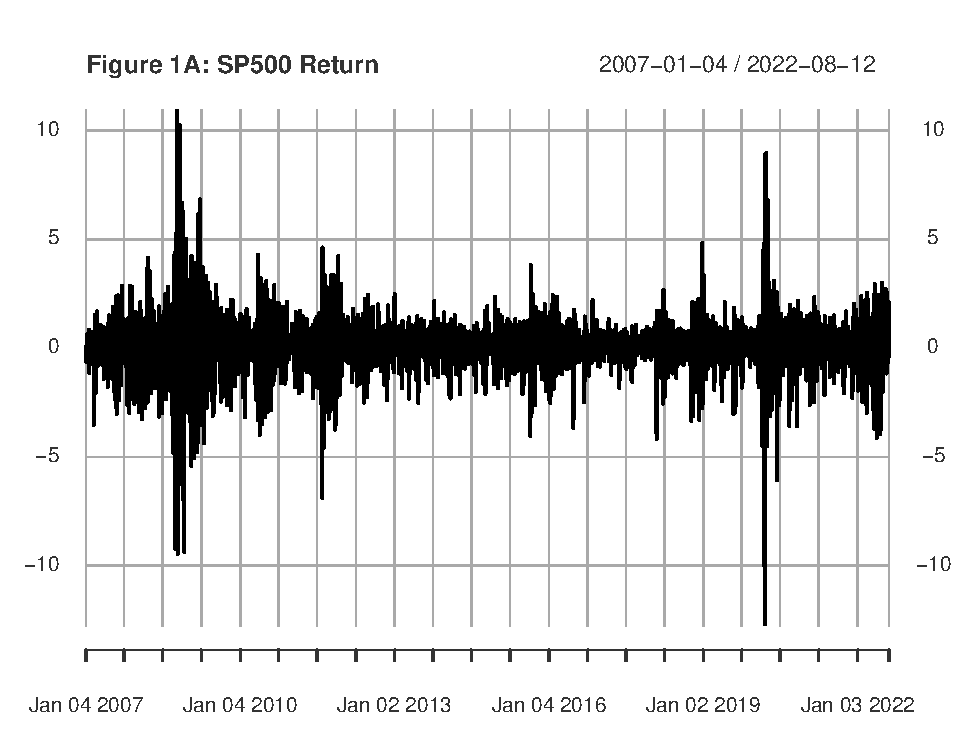
\includegraphics[width=1\linewidth]{bookdown-demo_files/figure-latex/ch7-figure1-1} 

}

\end{figure}\begin{figure}

{\centering 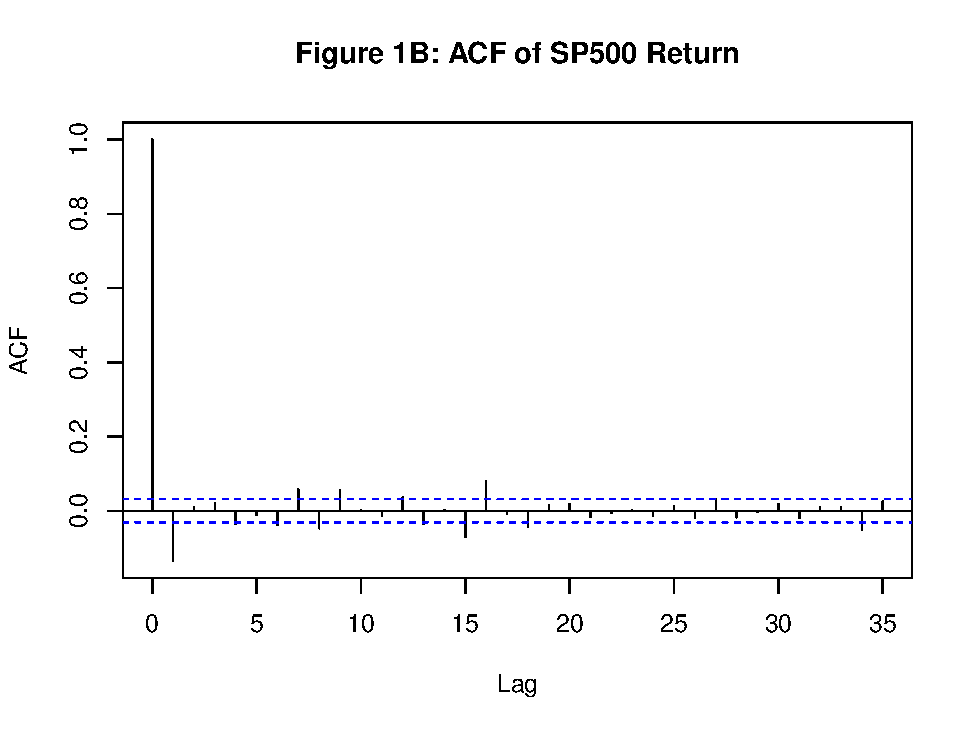
\includegraphics[width=1\linewidth]{bookdown-demo_files/figure-latex/ch7-figure1-2} 

}

\end{figure}\begin{figure}

{\centering 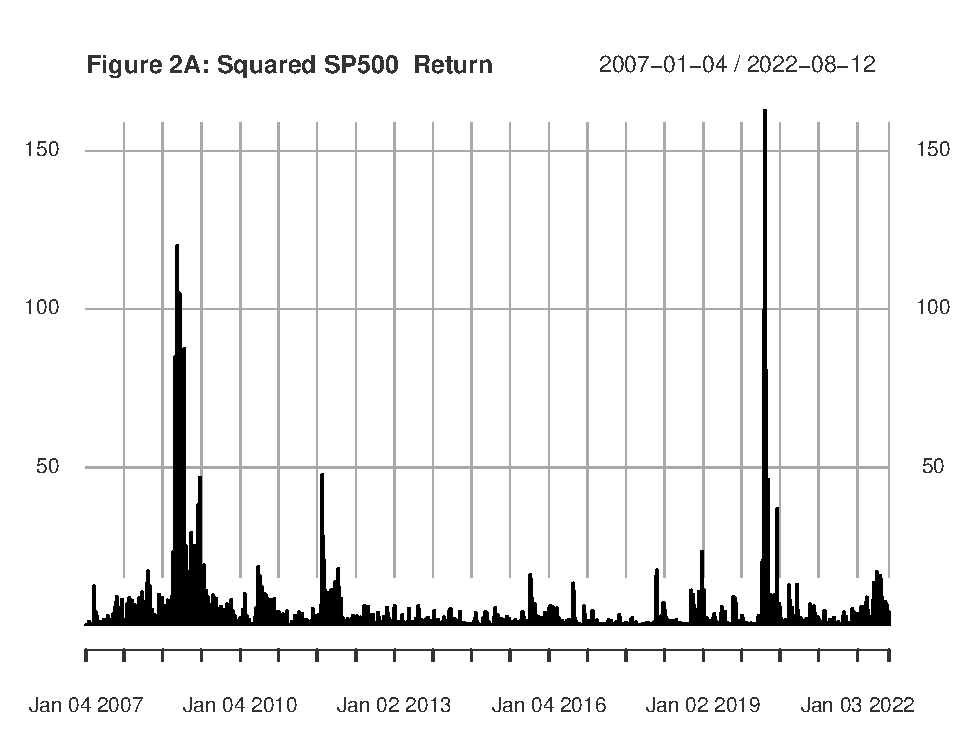
\includegraphics[width=1\linewidth]{bookdown-demo_files/figure-latex/ch7-figure1-3} 

}

\end{figure}\begin{figure}

{\centering 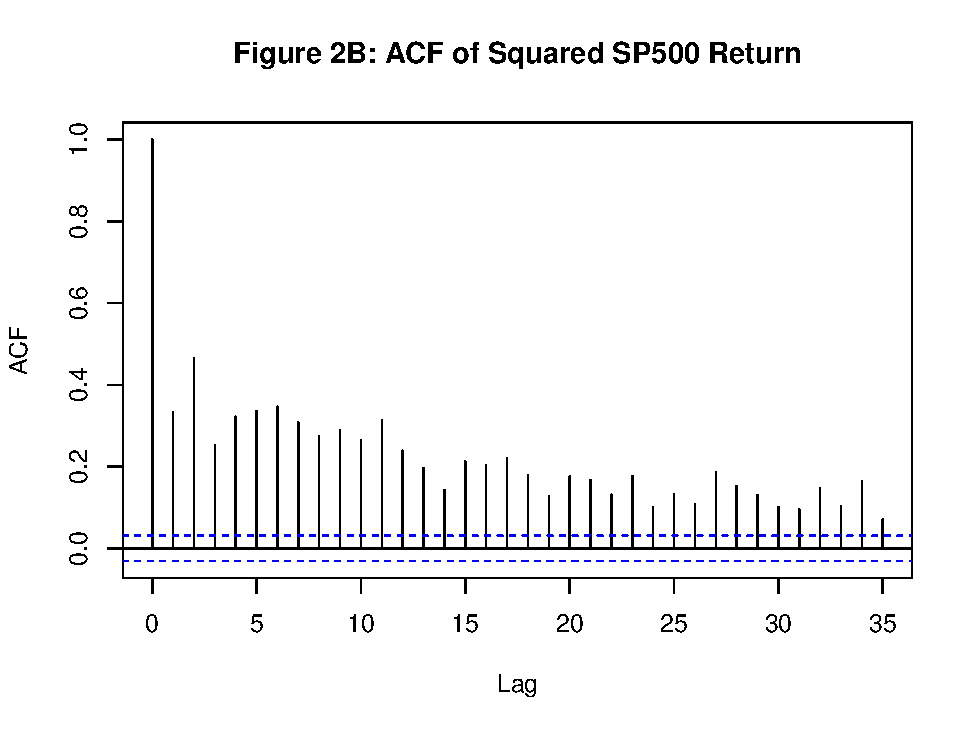
\includegraphics[width=1\linewidth]{bookdown-demo_files/figure-latex/ch7-figure1-4} 

}

\end{figure}

Focusing on the volatility, the plot of squared returns and its ACF establishes the following stylized facts:

\begin{enumerate}
\def\labelenumi{\arabic{enumi}.}
\item
  From Figure 2A, we observe that large values of squared returns cluster together, and small values of squared returns cluster together. That is periods of high volatility are followed by periods of high volatility and periods of low volatility are followed by periods of low volatility. This phenomenon is known as \textbf{volatility persistence} or \textbf{volatility clustering} in the fields of economics and finance.
\item
  A more direct evidence for volatility persistence can be inferred from the ACF plot of squared returns. From Figure 2B, we observe a strong positive serial correlation in squared returns.
\end{enumerate}

Hence, it is reasonable to assume that the variance of a financial time series may not be constant over time. Next we learn two classes of models that have been suggested to model conditional variance of a time series.

\hypertarget{archq-autoregressive-conditional-heteroscedasticiy-of-order-q}{%
\section{\texorpdfstring{ARCH(q): Autoregressive Conditional Heteroscedasticiy of order \(q\)}{ARCH(q): Autoregressive Conditional Heteroscedasticiy of order q}}\label{archq-autoregressive-conditional-heteroscedasticiy-of-order-q}}

Engle (1982) proposed a non-linear model for the conditional variance of a stationary time series where past squared shocks affect current volatility. For simplicity, let us assume that we are not interested in modeling the mean of the time series. Hence, our model for the mean is a constant value, \(\mu\). Then, an \(ARCH(1)\) model can be specified as follows:

\[\text{Mean Model:} \quad y_t = \mu +\epsilon_t \quad \text{where} \ \epsilon_t=\nu_t  \sigma_t \ \text{and} \ \nu_t\sim N(0,1)\]

\[\text{Variance Model:} \quad  \sigma_t^2=\omega +\alpha_1 \epsilon_{t-1}^2 \text{where} \ \omega>0 \ \text{and} \ \alpha_1>0 \]

In this model the unconditional variance of the time series is constant, but the conditional variance depends on the past squared error term. The variance model can be easily generalized to include \(q\) past shocks which gives us \(ARCH(q)\)

\[\text{Variance Model:} \quad  \sigma_t^2=\omega +\alpha_1 \epsilon_{t-1}^2+\alpha_2 \epsilon_{t-2}^2 +\alpha_3 \epsilon_{t-3}^2 +...+ \alpha_q \epsilon_{t-q}^2 \]
\[\text{where} \ \omega>0 \ \text{and} \ \alpha_i>0 \ \forall \ i\]

\hypertarget{garchpq-generalized-autoregressive-conditional-heteroscedasicity-of-order-p-and-q}{%
\section{\texorpdfstring{GARCH(p,q): Generalized Autoregressive Conditional Heteroscedasicity of order \(p\) and \(q\)}{GARCH(p,q): Generalized Autoregressive Conditional Heteroscedasicity of order p and q}}\label{garchpq-generalized-autoregressive-conditional-heteroscedasicity-of-order-p-and-q}}

A generalization of the above ARCH model was proposed by Bolerslev (1986) where the conditional variance in the current period depend on past squared shocks as well as past observations of the conditional variance. This model is known as \(GARCH\) which stands for generalized ARCH model. Formally, the variance equation of a \(GARCH(1,1)\) is given by:

\[\quad  \sigma_t^2=\omega +\alpha_1 \epsilon_{t-1}^2 +\beta_1 \sigma^2_{t-1} \quad \text{where} \ \omega>0, \ \alpha_1>0, \ \text{and} \ \beta_1>0 \]

In practice most models of volatility now use some version of GARCH(1,1) as it provides a more parsimonious model of volatility when compared to an ARCH(q) model. Following are few important properties of a standard GARCH(1,1) model:

\begin{enumerate}
\def\labelenumi{\roman{enumi}.}
\item
  Unconditional variance: The unconditional variance of \(y_t\) is still constant due to stationarity and is given by:
  \[\sigma^2_y = \frac{\omega}{1-\alpha_1-\beta_1}\]
\item
  Volatility persistence: the persistence is given by \(\alpha_1+\beta_1\).
\item
  Half-life measure: R is the number of periods it takes for the estimated volatility to converge to half of the unconditional variance of the time series.
\end{enumerate}

\hypertarget{extensions-of-standard-garch-model}{%
\section{Extensions of standard GARCH model}\label{extensions-of-standard-garch-model}}

There are two issues with the standard GARCH model that merits more discussion:

\begin{enumerate}
\def\labelenumi{\arabic{enumi}.}
\tightlist
\item
  In the standard GARCH framework, the effect of past shocks on volatility is symmetric. That is whether the observed shock is \textbf{negative} or \textbf{positive}, the effect on the volatility is the same.
  However, in the financial market another stylized fact is the asymmetric response of volatility to news. For instance, it is quite common to find that negative news increases volatility more than the reduction in volatility caused by positive news. One analytical tool to illustrate this point is the \textbf{news impact curve} where we plot the shock on the x-axis and estimated/predicted volatility from our GARCH model on the y-axis. Below I plot three types of news impact curves. In the first case, the curve is symmetric: negative and positive shocks have identical effect on volatility. In the second case, negative news has a bigger effect on volatility, and finally in the third case, positive news has a bigger effect on volatility.
\end{enumerate}

\begin{figure}

{\centering 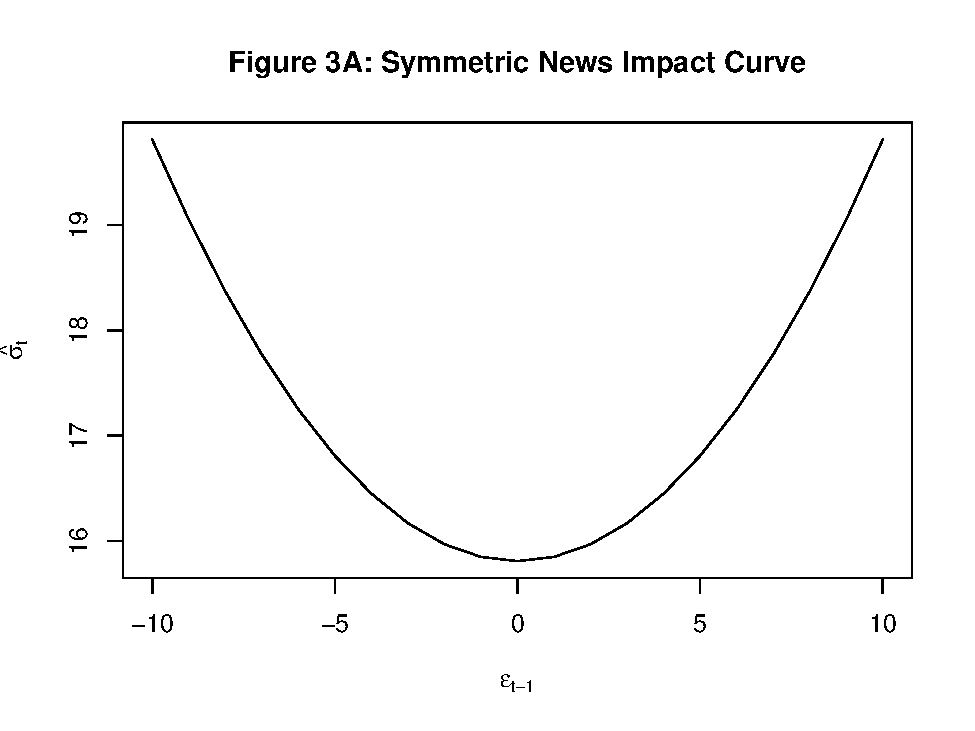
\includegraphics[width=1\linewidth]{bookdown-demo_files/figure-latex/ch7-figure2-1} 

}

\end{figure}\begin{figure}

{\centering 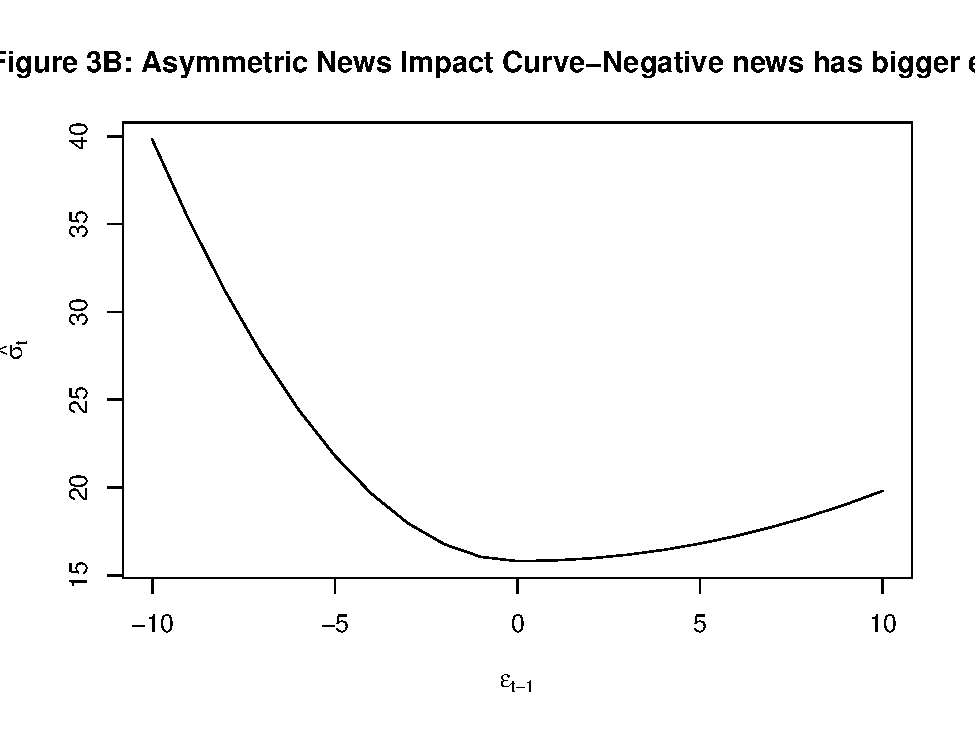
\includegraphics[width=1\linewidth]{bookdown-demo_files/figure-latex/ch7-figure2-2} 

}

\end{figure}\begin{figure}

{\centering 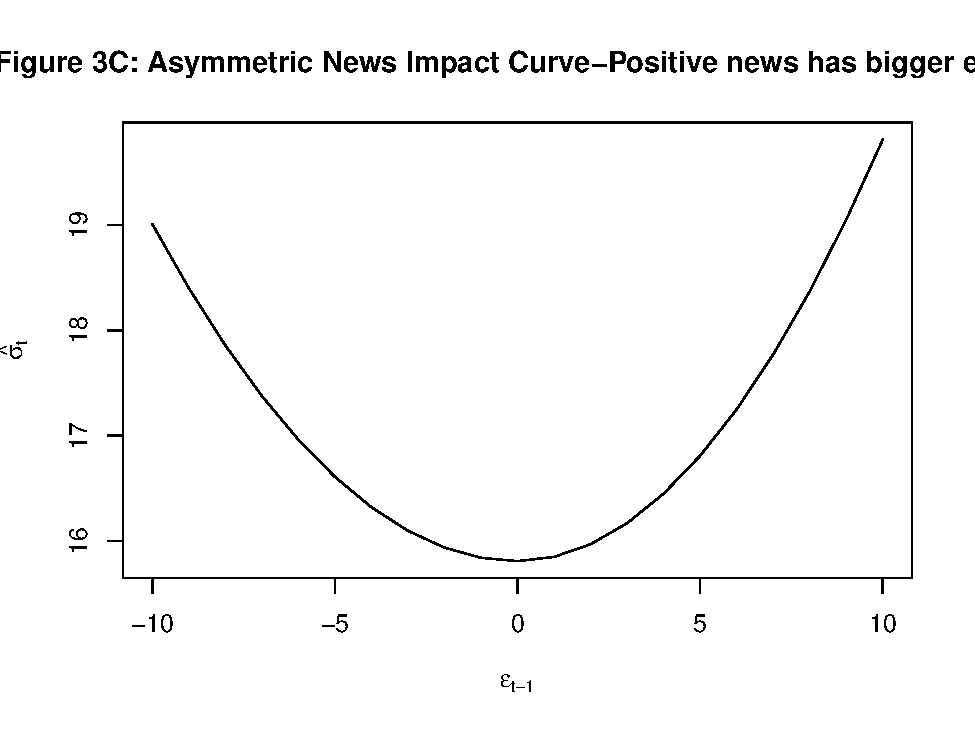
\includegraphics[width=1\linewidth]{bookdown-demo_files/figure-latex/ch7-figure2-3} 

}

\end{figure}

\begin{enumerate}
\def\labelenumi{\arabic{enumi}.}
\setcounter{enumi}{1}
\tightlist
\item
  Because these models are models of variance which cannot be negative, the estimation of these models imposes non-negativity condition on all estimated parameters. For instance, in \(GARCH(1,1)\) we assume that \(\omega, \alpha_1, \ \text{and} \ \beta_1\) are all positive.
\end{enumerate}

\hypertarget{gjr-garch11}{%
\subsection{GJR-GARCH(1,1)}\label{gjr-garch11}}

Glosten, Jagannathan, and Runkle (1993) proposed a variation of the standard GARCH model that incorporates the asymmetry of the impact of news on volatility. The resulting model is called GJR-GARCH and it addresses the first of the issues listed above. Formally, the variance equation of the GJR-GARCH(1,1) is given by:

\[ \sigma_t^2=\omega+\alpha_1 \epsilon^2_{t-1}+\beta_1 \sigma^2_{t-1}+\gamma_1 D_{t-1}\epsilon^2_{t-1}\]

where \(D_{t-1}=1\) if \(\epsilon_{t-1}<0\) and \(0\) otherwise. Hence, now the effect of \(\epsilon^2_{t-1}\) on volatility is \(\alpha_1+\gamma_1\) for negative shocks and \(\alpha_1\) for positive shocks. The news impact curve from this model will be asymmetric. The persistence from this model will also be affected by \(\gamma_1\). Specfically for the GJR-GARCH(1,1) model,

\begin{enumerate}
\def\labelenumi{\arabic{enumi}.}
\item
  Persistence: \(\alpha_1+\beta_1 +\frac{\gamma_1}{2}\)
\item
  Unconditional variance: \[\sigma^2_y = \frac{\omega}{1-\alpha_1-\beta_1-\frac{\gamma_1}{2}}\]
\end{enumerate}

\hypertarget{exponential-garch-or-egarch11}{%
\subsection{Exponential GARCH or EGARCH(1,1)}\label{exponential-garch-or-egarch11}}

Exponential GARCH model by Nelson (1991) accounts for both the issues outlined above. It allows for asymmetric effects of shocks and also does not require the non-negativity constraints. More importantly, it also accounts for different effect of shocks of different magnitude, and hence provides an estimate of the \textbf{size effect}. Formally, the variance equation for EGARCH(1,1) is given by:

\[ln(\sigma^2_{t-1})=\omega+ \alpha_1 z_{t-1} +\gamma_1 (|z_{t-1}|-E|z_{t-1}|) +\beta_1\sigma^2_{t-1}\]

where \(z_t=\frac{\epsilon_t}{\sigma_t}\) is the standardized error term. Here, \(\alpha_1\) captures the sign effect and \(\gamma_1\) captures the size effect. A common finding is that negative news and larger shocks have bigger effect on volatility. Accordingly, we often find in empirical applications of EGARCH that \(\alpha_1<0\) and \(\gamma_1>0\). For this model, we have

\begin{enumerate}
\def\labelenumi{\arabic{enumi}.}
\item
  Persistence: \(\beta_1\)
\item
  Unconditional variance: \[\sigma^2_y = \frac{\omega}{1-\beta_1}\]
\end{enumerate}

\hypertarget{application-of-garch-model-estimating-volatility-of-sp500-return}{%
\section{Application of GARCH model: Estimating volatility of SP500 return}\label{application-of-garch-model-estimating-volatility-of-sp500-return}}

In this application, we will estimate the volatility underlying SP500 returns (Figure 1A and Figure 2A). The first step is to test whether squared returns have ARCH effects i.e, whether there is any evidence for time-varying volatility in our data. For this purpose we will use Engle's ARCH test. Consider our constant mean model:

\[y_t=\mu +\epsilon_t\]

We can estimate the above model by OLS and obtain residuals \(e_t=y_t-\hat{y_t}\). The test for ARCH effects is based on the idea that is there is conditional hetroscedasiticity in our data then the squared residuals will have serial correlation. The ARCH test involves estimating the following regression:

\[e^2_t= \beta_0 +\beta_1 e^2_{t-1} + \beta_2 e^2_{t-2}+...+ \beta_p e^2_{t-p} + u_t\]

Then, the test for ARCH effects is given by:

\[H_0: \beta_1=\beta_2=...=\beta_p=0 \ \Rightarrow \text{no ARCH effects}\]
\[ H_A: \text{Not} \ H_0\]

In R, we use a package called \textbf{aTSA} to implement this test.The function is called \textbf{arch.test()}. Figure 7.1 below shows the results of this test for our data.

\begin{Shaded}
\begin{Highlighting}[]
\KeywordTok{library}\NormalTok{(aTSA)}
\KeywordTok{library}\NormalTok{(forecast)}

\NormalTok{fit=}\KeywordTok{arima}\NormalTok{(y, }\KeywordTok{c}\NormalTok{(}\DecValTok{0}\NormalTok{,}\DecValTok{0}\NormalTok{,}\DecValTok{0}\NormalTok{))}

\KeywordTok{arch.test}\NormalTok{(fit)}
\end{Highlighting}
\end{Shaded}

\begin{verbatim}
## ARCH heteroscedasticity test for residuals 
## alternative: heteroscedastic 
## 
## Portmanteau-Q test: 
##      order   PQ p.value
## [1,]     4 1074       0
## [2,]     8 2267       0
## [3,]    12 3556       0
## [4,]    16 4150       0
## [5,]    20 4857       0
## [6,]    24 5482       0
## Lagrange-Multiplier test: 
##      order   LM p.value
## [1,]     4 2193       0
## [2,]     8  692       0
## [3,]    12  402       0
## [4,]    16  272       0
## [5,]    20  215       0
## [6,]    24  170       0
\end{verbatim}

\begin{figure}
\centering
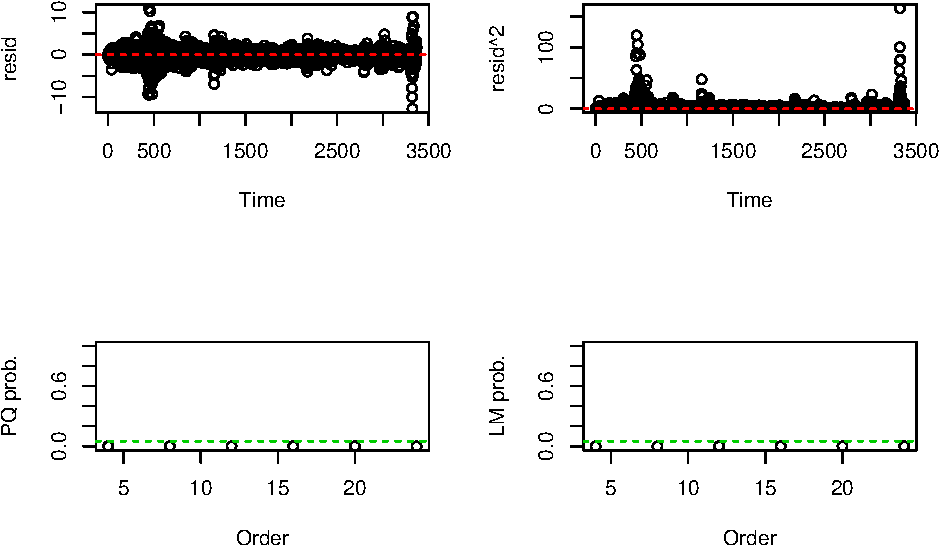
\includegraphics{bookdown-demo_files/figure-latex/table1-1.pdf}
\caption{\label{fig:table1}ARCH LM test}
\end{figure}

We find strong evidence for ARCH effects in our data as the null hypothesis of no ARCH effects is rejected at different orders of serial correlation in squared residuals. Next we estimate three types of GARCH(1,1) models using the \textbf{rugarch} package. Tables 7.1A-7.1D below show the estimated parameters of these three models. The news impact curve for these 3 classes of GARCH model are plotted in Figure 2-4 below. Finally, the estimated conditional volatility from the three models are plotted along with the return in Figures 5-7. We find that there is strong evidence for the sign effect with negative news having a bigger effect on volatility as indicated by the positive value for \(\gamma_1\) in GJR-GARCH and negative value of \(\alpha_1\) in EGARCH. Further, in the EGARCH model we find evidence for the size effect as indicated by positive value for \(\gamma_1\). These findings are confirmed by the asymmetric news impact curves for the GJR-GARCH and EGARCH models.

\begin{table}[t]

\caption{\label{tab:unnamed-chunk-11}(A) Estimated GARCH(1,1)}
\centering
\begin{tabular}{l|r|r|r|r}
\hline
  &  Estimate &  Std. Error &  t value & Pr(>|t|)\\
\hline
mu & 0.068 & 0.014 & 4.916 & 0\\
\hline
omega & 0.026 & 0.004 & 6.653 & 0\\
\hline
alpha1 & 0.132 & 0.013 & 10.049 & 0\\
\hline
beta1 & 0.848 & 0.013 & 63.704 & 0\\
\hline
\end{tabular}
\end{table}

\begin{table}[t]

\caption{\label{tab:unnamed-chunk-11}(B) Estimated GJR-GARCH(1,1)}
\centering
\begin{tabular}{l|r|r|r|r}
\hline
  &  Estimate &  Std. Error &  t value & Pr(>|t|)\\
\hline
mu & 0.029 & 0.014 & 2.108 & 0.035\\
\hline
omega & 0.027 & 0.003 & 7.975 & 0.000\\
\hline
alpha1 & 0.000 & 0.013 & 0.000 & 1.000\\
\hline
beta1 & 0.864 & 0.013 & 66.157 & 0.000\\
\hline
gamma1 & 0.219 & 0.023 & 9.348 & 0.000\\
\hline
\end{tabular}
\end{table}

\begin{table}[t]

\caption{\label{tab:unnamed-chunk-11}(C) Estimated EGARCH(1,1)}
\centering
\begin{tabular}{l|r|r|r|r}
\hline
  &  Estimate &  Std. Error &  t value & Pr(>|t|)\\
\hline
mu & 0.031 & 0.014 & 2.293 & 0.022\\
\hline
omega & 0.000 & 0.004 & -0.117 & 0.907\\
\hline
alpha1 & -0.178 & 0.013 & -13.380 & 0.000\\
\hline
beta1 & 0.969 & 0.004 & 265.865 & 0.000\\
\hline
gamma1 & 0.158 & 0.015 & 10.878 & 0.000\\
\hline
\end{tabular}
\end{table}

\begin{table}[t]

\caption{\label{tab:unnamed-chunk-11}(D) Persistence, Unconditional Variance, and Half-life}
\centering
\begin{tabular}{l|r|r|r}
\hline
  & GARCH(1,1) & GJR-GARCH(1,1) & EGARCH(1,1)\\
\hline
Persistence & 0.980 & 0.974 & 0.969\\
\hline
Unconditional Variance & 1.336 & 1.026 & 0.987\\
\hline
Half-life & 34.759 & 26.085 & 21.911\\
\hline
\end{tabular}
\end{table}

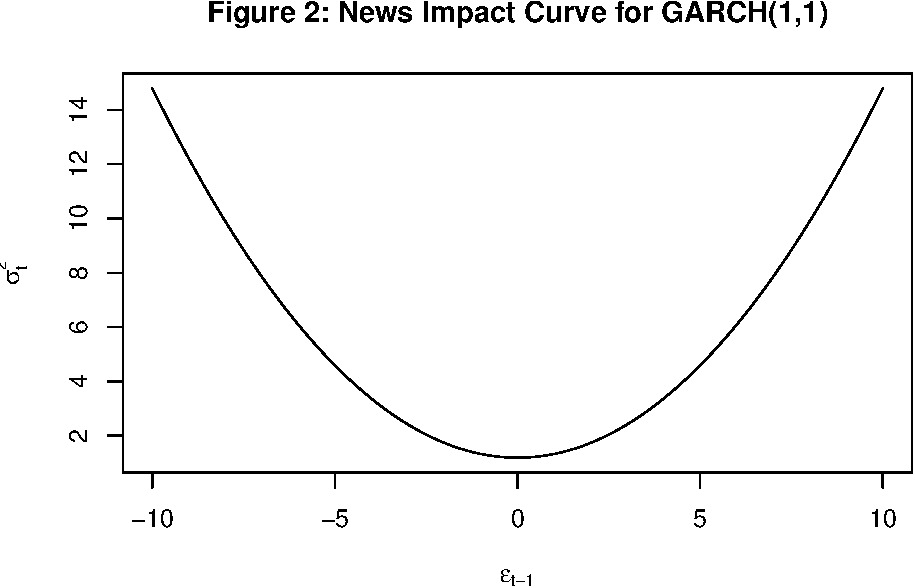
\includegraphics{bookdown-demo_files/figure-latex/unnamed-chunk-11-1.pdf} 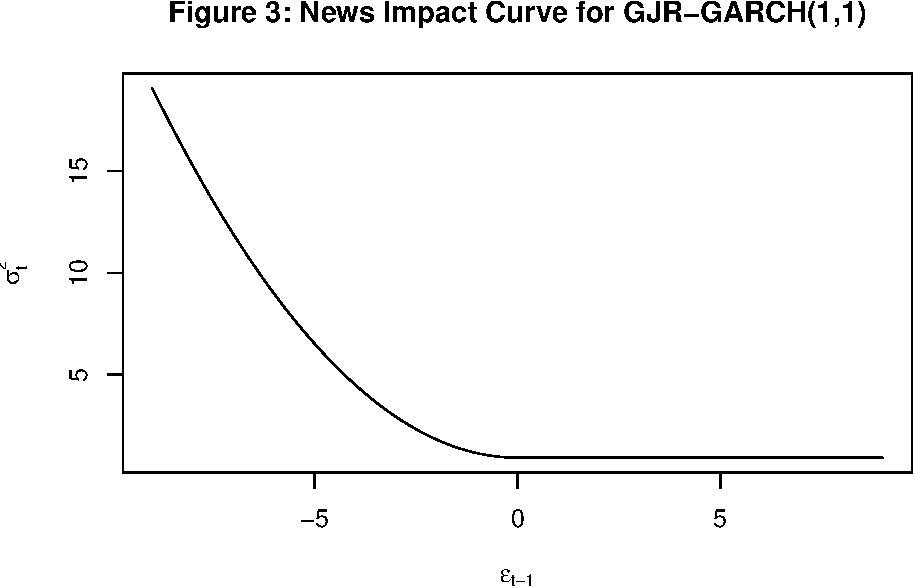
\includegraphics{bookdown-demo_files/figure-latex/unnamed-chunk-11-2.pdf} 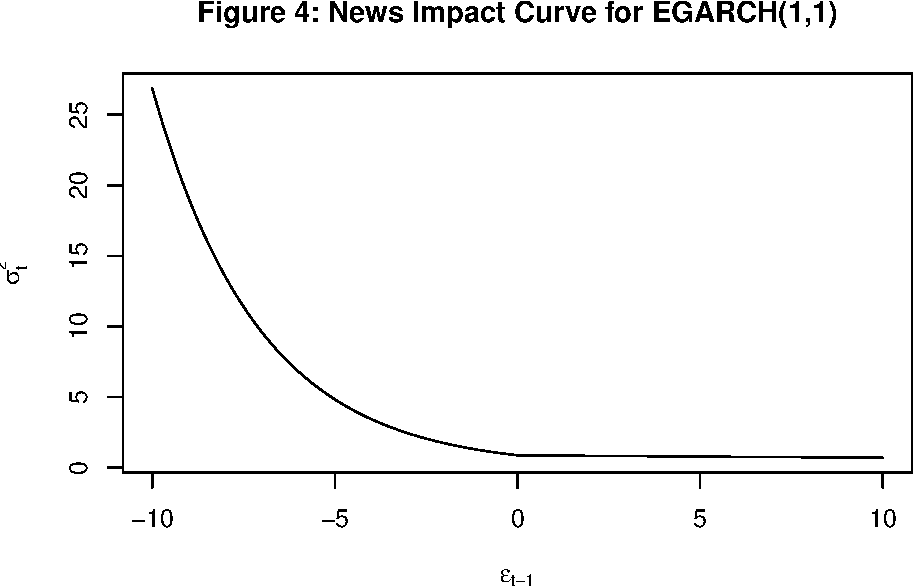
\includegraphics{bookdown-demo_files/figure-latex/unnamed-chunk-11-3.pdf} 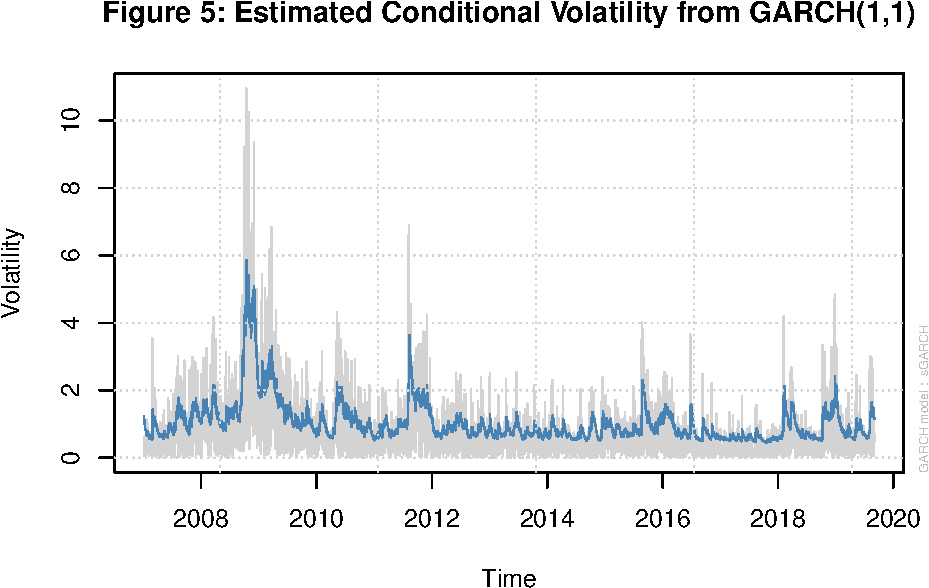
\includegraphics{bookdown-demo_files/figure-latex/unnamed-chunk-11-4.pdf} 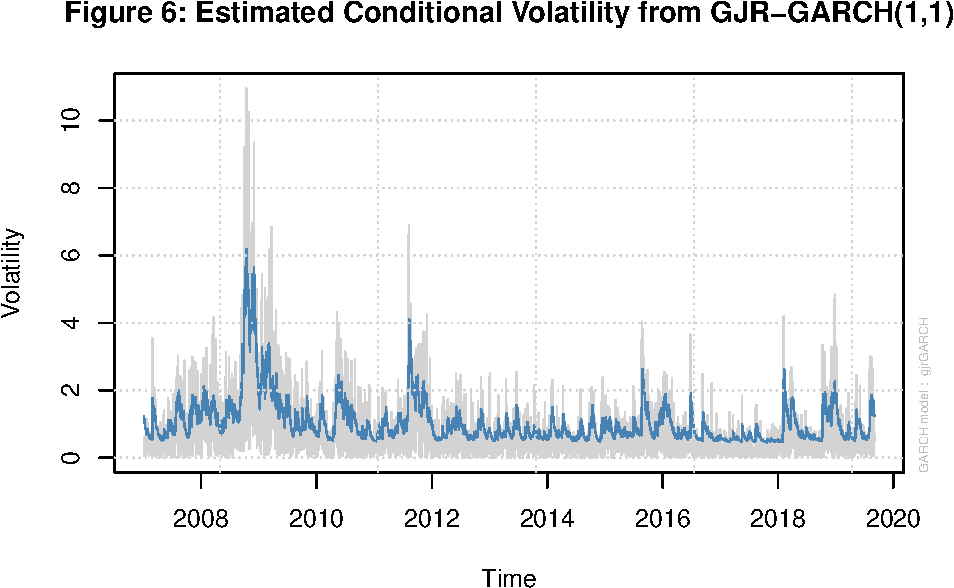
\includegraphics{bookdown-demo_files/figure-latex/unnamed-chunk-11-5.pdf} 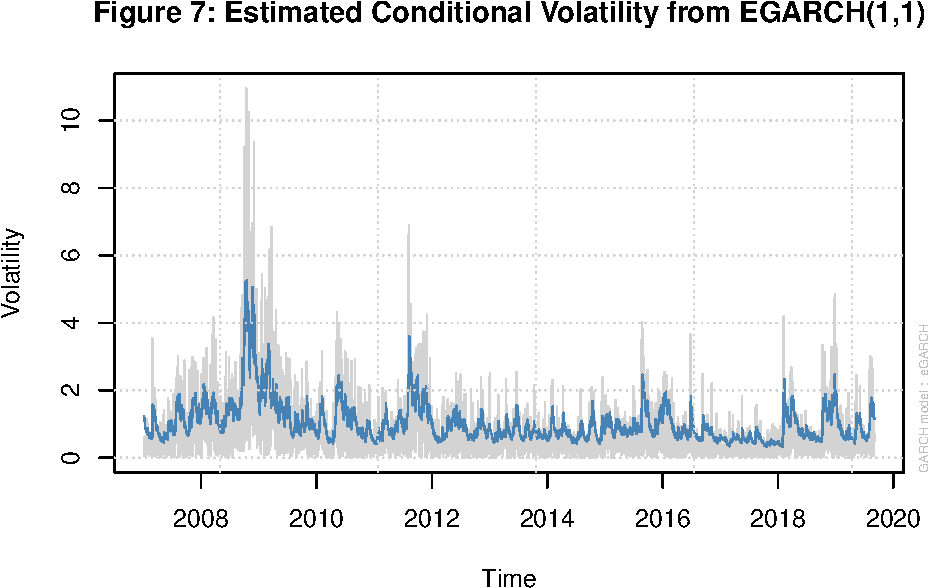
\includegraphics{bookdown-demo_files/figure-latex/unnamed-chunk-11-6.pdf}

Finally, these models can also be used to forecast the volatility of SP500. Figure 8 below shows this forecast for the next 7 days from the EGARCH(1.1) model.

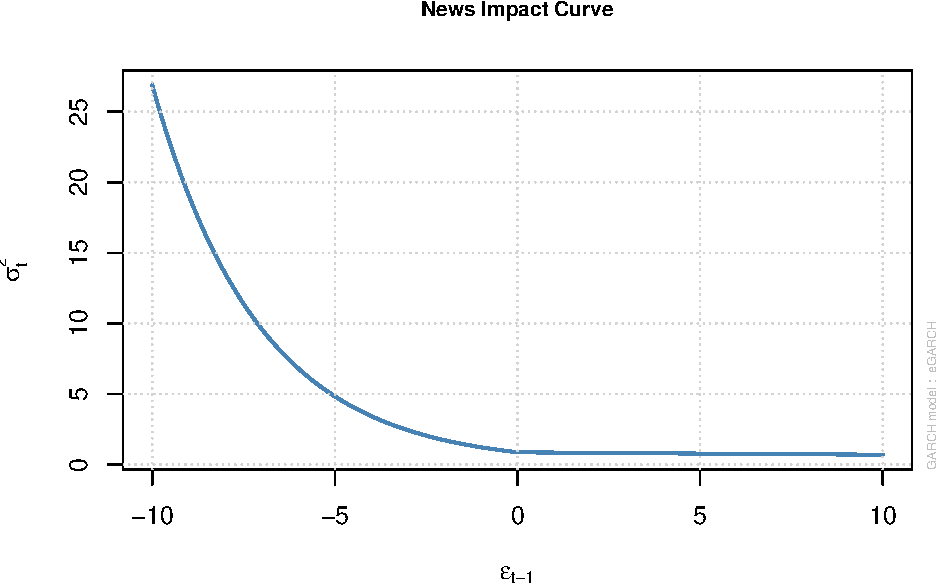
\includegraphics{bookdown-demo_files/figure-latex/unnamed-chunk-12-1.pdf} 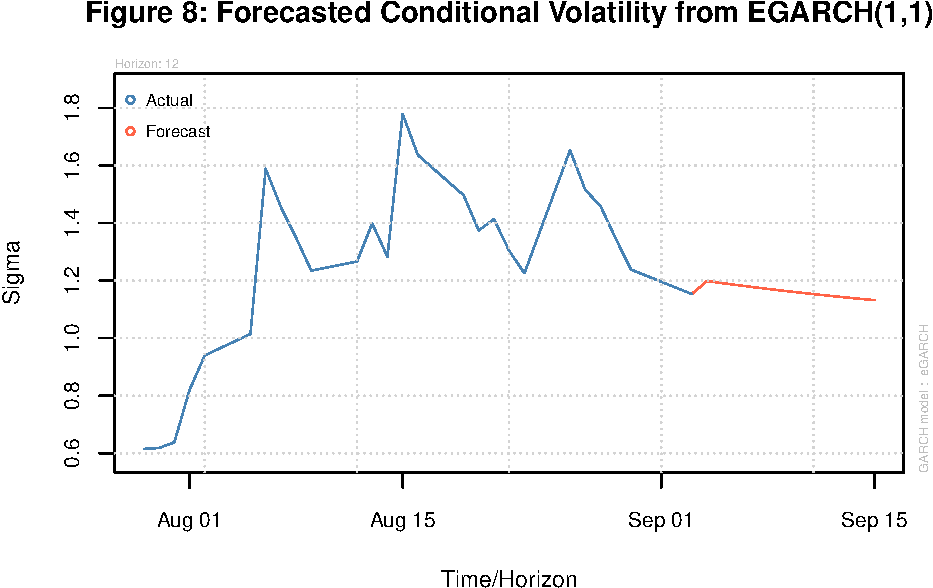
\includegraphics{bookdown-demo_files/figure-latex/unnamed-chunk-12-2.pdf}

\bibliography{book.bib,packages.bib}


\end{document}
